\documentclass[12pt,(landscape,a4paper),(portrait,a4paper)]{article}
\usepackage{lmodern}
\usepackage{amssymb,amsmath}
\usepackage{ifxetex,ifluatex}
\usepackage{fixltx2e} % provides \textsubscript
\ifnum 0\ifxetex 1\fi\ifluatex 1\fi=0 % if pdftex
  \usepackage[T1]{fontenc}
  \usepackage[utf8]{inputenc}
\else % if luatex or xelatex
  \ifxetex
    \usepackage{mathspec}
  \else
    \usepackage{fontspec}
  \fi
  \defaultfontfeatures{Ligatures=TeX,Scale=MatchLowercase}
\fi
% use upquote if available, for straight quotes in verbatim environments
\IfFileExists{upquote.sty}{\usepackage{upquote}}{}
% use microtype if available
\IfFileExists{microtype.sty}{%
\usepackage{microtype}
\UseMicrotypeSet[protrusion]{basicmath} % disable protrusion for tt fonts
}{}
\usepackage[margin=1in]{geometry}
\usepackage{hyperref}
\hypersetup{unicode=true,
            pdftitle={计量经济学Eviews实验指导书},
            pdfauthor={胡华平},
            pdfborder={0 0 0},
            breaklinks=true}
\urlstyle{same}  % don't use monospace font for urls
\usepackage{longtable,booktabs}
\usepackage{graphicx,grffile}
\makeatletter
\def\maxwidth{\ifdim\Gin@nat@width>\linewidth\linewidth\else\Gin@nat@width\fi}
\def\maxheight{\ifdim\Gin@nat@height>\textheight\textheight\else\Gin@nat@height\fi}
\makeatother
% Scale images if necessary, so that they will not overflow the page
% margins by default, and it is still possible to overwrite the defaults
% using explicit options in \includegraphics[width, height, ...]{}
\setkeys{Gin}{width=\maxwidth,height=\maxheight,keepaspectratio}
\IfFileExists{parskip.sty}{%
\usepackage{parskip}
}{% else
\setlength{\parindent}{0pt}
\setlength{\parskip}{6pt plus 2pt minus 1pt}
}
\setlength{\emergencystretch}{3em}  % prevent overfull lines
\providecommand{\tightlist}{%
  \setlength{\itemsep}{0pt}\setlength{\parskip}{0pt}}
\setcounter{secnumdepth}{5}
% Redefines (sub)paragraphs to behave more like sections
\ifx\paragraph\undefined\else
\let\oldparagraph\paragraph
\renewcommand{\paragraph}[1]{\oldparagraph{#1}\mbox{}}
\fi
\ifx\subparagraph\undefined\else
\let\oldsubparagraph\subparagraph
\renewcommand{\subparagraph}[1]{\oldsubparagraph{#1}\mbox{}}
\fi

%%% Use protect on footnotes to avoid problems with footnotes in titles
\let\rmarkdownfootnote\footnote%
\def\footnote{\protect\rmarkdownfootnote}

%%% Change title format to be more compact
\usepackage{titling}

% Create subtitle command for use in maketitle
\newcommand{\subtitle}[1]{
  \posttitle{
    \begin{center}\large#1\end{center}
    }
}

\setlength{\droptitle}{-2em}
  \title{计量经济学Eviews实验指导书}
  \pretitle{\vspace{\droptitle}\centering\huge}
  \posttitle{\par}
\subtitle{Lab 6 异方差模型的诊断和矫正}
  \author{胡华平}
  \preauthor{\centering\large\emph}
  \postauthor{\par}
  \predate{\centering\large\emph}
  \postdate{\par}
  \date{2018/4/13}

\usepackage{xeCJK}
\setCJKmainfont{楷体}  % 字体可以更换
\setmainfont{Georgia} % 設定英文字型
\setromanfont{Georgia} % 字型
\setmonofont{Courier New}

%设置版式 垂直或水平
% You know, for landscape
\usepackage{lscape}
\usepackage{pdfpages}


% Make new page before each section
\let\stdsection\section
\renewcommand\section{\newpage\stdsection}

% pandoc does not parse latex env - https://groups.google.com/forum/?fromgroups=#!topic/pandoc-discuss/oZETB5Ii1Cw
\newcommand{\blandscape}{\begin{landscape}}
\newcommand{\elandscape}{\end{landscape}}

\begin{document}
\maketitle

\renewcommand{\figurename}{图}
\renewcommand{\contentsname}{目录}
\renewcommand{\tablename}{表}


%% maxwidth is the original width if it's less than linewidth
%% otherwise use linewidth (to make sure the graphics do not exceed the margin)
\makeatletter
\def\maxwidth{ %
  \ifdim\Gin@nat@width>\linewidth
    \linewidth
  \else
    \Gin@nat@width
  \fi
}
\makeatother

{
\setcounter{tocdepth}{5}
\tableofcontents
}
\hypertarget{heteroskedasticity}{%
\section{异方差的诊断和矫正}\label{heteroskedasticity}}

\newpage

\subsection{实验目的及要求}

\begin{itemize}
\tightlist
\item
  \textbf{目的}:掌握异方差问题的检验与处理方法。
\item
  \textbf{要求}:在老师指导下完成计量经济模型的异方差检验,并对存在异方差的模型进行修正,最终得到正确的分析结果。
\end{itemize}

\subsection{实验原理}

\begin{itemize}
\tightlist
\item
  对于不同的样本点,随机误差项的方差不再是常数,而互不相同,则认为出现了异方差性。
\item
  异方差的实质表现为随机误差项的方差随着解释变量(引起异方差的解释变量)观测值的变化而变化。
\item
  对于出现异方差的原模型主要采用校正其异方差,再对校正后的模型采用普通最小二乘法估计。
\end{itemize}

\subsection{实验内容}

\begin{enumerate}
\def\labelenumi{\arabic{enumi}.}
\item
  采用最小二乘法建立主回归模型
\item
  侦查模型是否存在异方差问题

  \begin{enumerate}
  \def\labelenumii{\arabic{enumii})}
  \tightlist
  \item
    非正式检验方法(图形检验法):

    \begin{itemize}
    \tightlist
    \item
      残差趋势图(dot plot)
    \item
      残差散点图(scatter plot)
    \end{itemize}
  \item
    正式检验方法

    \begin{itemize}
    \tightlist
    \item
      Park检验法
    \item
      Glejser检验法
    \item
      BPG检验法
    \item
      White检验法
    \end{itemize}
  \end{enumerate}
\item
  在发现存在异方差的基础上,对原模型进行异方差问题的处理:

  \begin{enumerate}
  \def\labelenumii{\arabic{enumii})}
  \tightlist
  \item
    使用加权最小二乘法校正异方差\\
  \item
    使用White校正法解决异方差
  \end{enumerate}
\end{enumerate}

\subsubsection{实验背景------汽车油耗}

\textbf{汽车油耗数据}:表\ref{tab:data-car}给出给出了81辆汽车在Y单位油耗的行驶里程数(英里/加仑),X2最高时速(英里/小时),X3发动机马力,X4汽车空间(立方英尺),X5车身重量(百磅)等方面的数据。

\begin{table}

\caption{\label{tab:data-car}汽车单位油耗里程数据(n=81)}
\centering
\begin{tabular}[t]{rrrrrr}
\toprule
obs & Y & X2 & X3 & X4 & X5\\
\midrule
1 & 65.4 & 96 & 49 & 89 & 17.5\\
2 & 56.0 & 97 & 55 & 92 & 20.0\\
3 & 55.9 & 97 & 55 & 92 & 20.0\\
4 & 49.0 & 105 & 70 & 92 & 20.0\\
5 & 46.5 & 96 & 53 & 92 & 20.0\\
\addlinespace
77 & 18.1 & 165 & 322 & 50 & 45.0\\
78 & 17.2 & 140 & 238 & 115 & 45.0\\
79 & 17.0 & 147 & 263 & 50 & 45.0\\
80 & 16.7 & 157 & 295 & 119 & 45.0\\
81 & 13.2 & 130 & 236 & 107 & 55.0\\
\bottomrule
\end{tabular}
\end{table}

变量说明见表\ref{tab:label-car}:

\begin{table}

\caption{\label{tab:label-car}变量定义及说明}
\centering
\begin{tabular}[t]{l|l}
\hline
variable & label\\
\hline
obs & 汽车品牌序号\\
\hline
Y & 单位油耗的行驶里程数(英里/加仑)\\
\hline
X2 & 最高时速(英里/小时)\\
\hline
X3 & 发动机马力\\
\hline
X4 & 汽车空间(立方英尺)\\
\hline
X5 & 车身重量(百磅)\\
\hline
\end{tabular}
\end{table}

~

请考虑如下样本回归模型:

\begin{equation}
Y_i=\beta_1+\beta_2X_{2i}+\beta_3X_{3i}+\beta_4X_{4i}+\beta_5X_{5i}+e_{i} \label{eq:M0-car}
\end{equation}

\subsection{主要实验步骤}

\subsubsection{导入数据并进行预处理}

\begin{itemize}
\tightlist
\item
  目标:
\item
  思路:
\item
  新建Eviews工作文件(见图\ref{fig:fig-load-data})

  \begin{itemize}
  \tightlist
  \item
    提示:Excel数据,每个同学的Y数据都不同,找到自己学号对应下的Y
  \item
    Eviews菜单操作:

    \begin{enumerate}
    \def\labelenumi{\alph{enumi}.}
    \tightlist
    \item
      依次操作:File\(\Rightarrow\)New\(\Rightarrow\)Workfile
    \item
      进行workfile create引导设置:

      \begin{itemize}
      \tightlist
      \item
        workfile structure type: \texttt{unstructured/undatede}
      \item
        data range:81
      \item
        workfile names(optional):

        \begin{itemize}
        \tightlist
        \item
          WF: \texttt{car}(\textbf{建议命名})
        \item
          Page: \texttt{mileage}(\textbf{建议命名})
        \end{itemize}
      \end{itemize}
    \end{enumerate}
  \end{itemize}
\item
  Eviews导入数据

  \begin{itemize}
  \tightlist
  \item
    提示:Excel数据,每个同学的Y数据都不同,找到自己学号对应下的Y数据(X数据所有同学都一样)\\
  \item
    菜单操作(Excel和Eviews):

    \begin{enumerate}
    \def\labelenumi{\alph{enumi}.}
    \tightlist
    \item
      Excel找到数据。Excel表格中仅保留自己需要的数据(obs, Y, X2, X3,
      X4, X5)
    \item
      Eviews导入数据。File\(\Rightarrow\)Import\(\Rightarrow\)Import
      From File:\texttt{d:/econometrics/data/Lab6-car.xlsx}
    \end{enumerate}
  \end{itemize}
\end{itemize}

\begin{figure}

{\centering 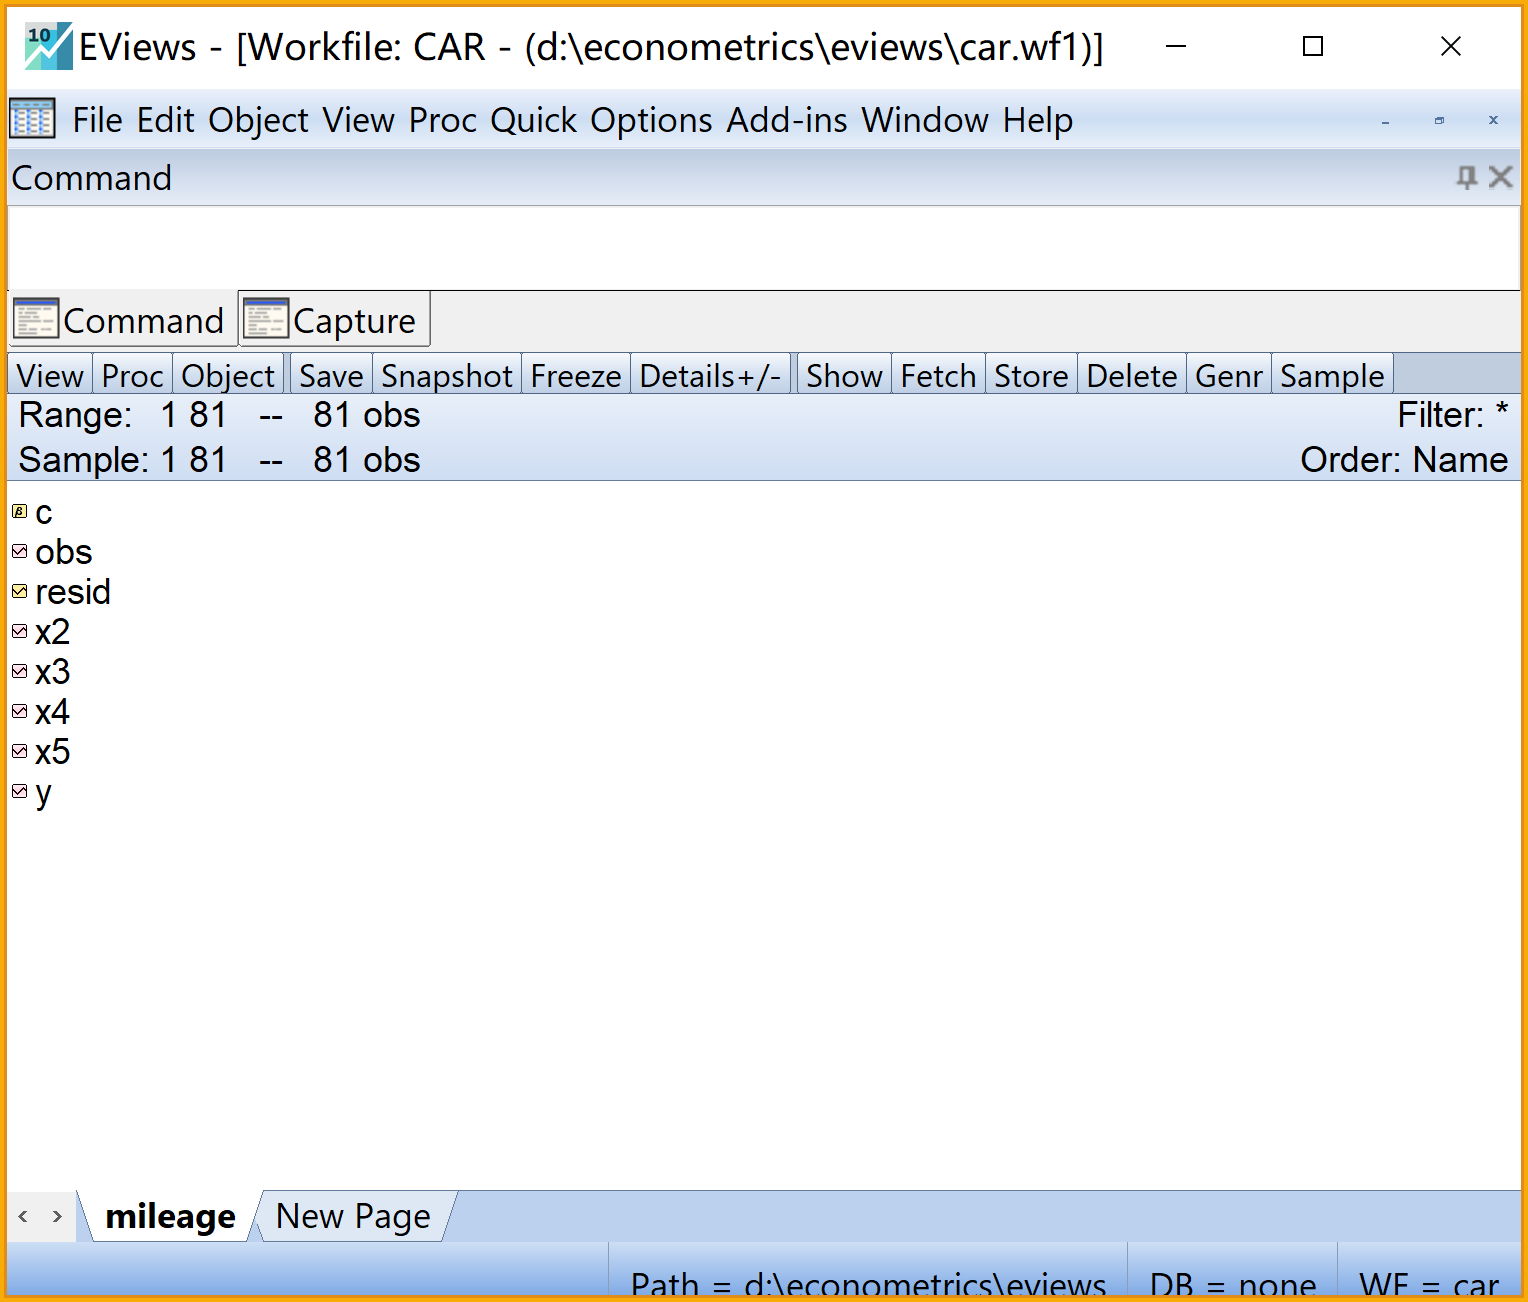
\includegraphics[width=21.22in]{picture/lab6-heteroskedasticity/1-load-data} 

}

\caption{导入数据的Eviews视窗}\label{fig:fig-load-data}
\end{figure}

\hypertarget{main-model}{%
\subsubsection{采用最小二乘法建立主回归模型}\label{main-model}}

\begin{itemize}
\tightlist
\item
  目标:
\item
  思路:
\item
  提示:主回归模型为
\end{itemize}

\[Y_t=\hat{\beta}_1+\hat{\beta}_2X_{2i}+\hat{\beta}_3X_{3i}+\hat{\beta}_4X_{4i}+\hat{\beta}_5X_{5i}+e_{i}\]

\begin{itemize}
\tightlist
\item
  Eviews菜单操作(见图\ref{fig:fig-eq-m0}):

  \begin{enumerate}
  \def\labelenumi{\arabic{enumi})}
  \item
    依次选择\(\Rightarrow\)Quick\(\Rightarrow\)Estimation Equation\\
  \item
    引导设置Equation Estimation\(\Rightarrow\)specification

    \begin{enumerate}
    \def\labelenumii{\alph{enumii}.}
    \tightlist
    \item
      Equation specification:输入命令 Y c X2 X3 X4 X5
    \item
      Estimation settings:

      \begin{itemize}
      \tightlist
      \item
        Method: 下拉选择\texttt{LS\ -\ Least\ Squares\ (NLS\ and\ ARMA)}
      \item
        Sample: \textbf{默认设置}
      \end{itemize}
    \item
      点击\texttt{OK}\\
    \end{enumerate}
  \item
    模型命名:建议为\texttt{eq\_m0}

    主回归分析结果见图\ref{fig:fig-eq-m0-report}:
  \end{enumerate}
\end{itemize}

\begin{figure}

{\centering 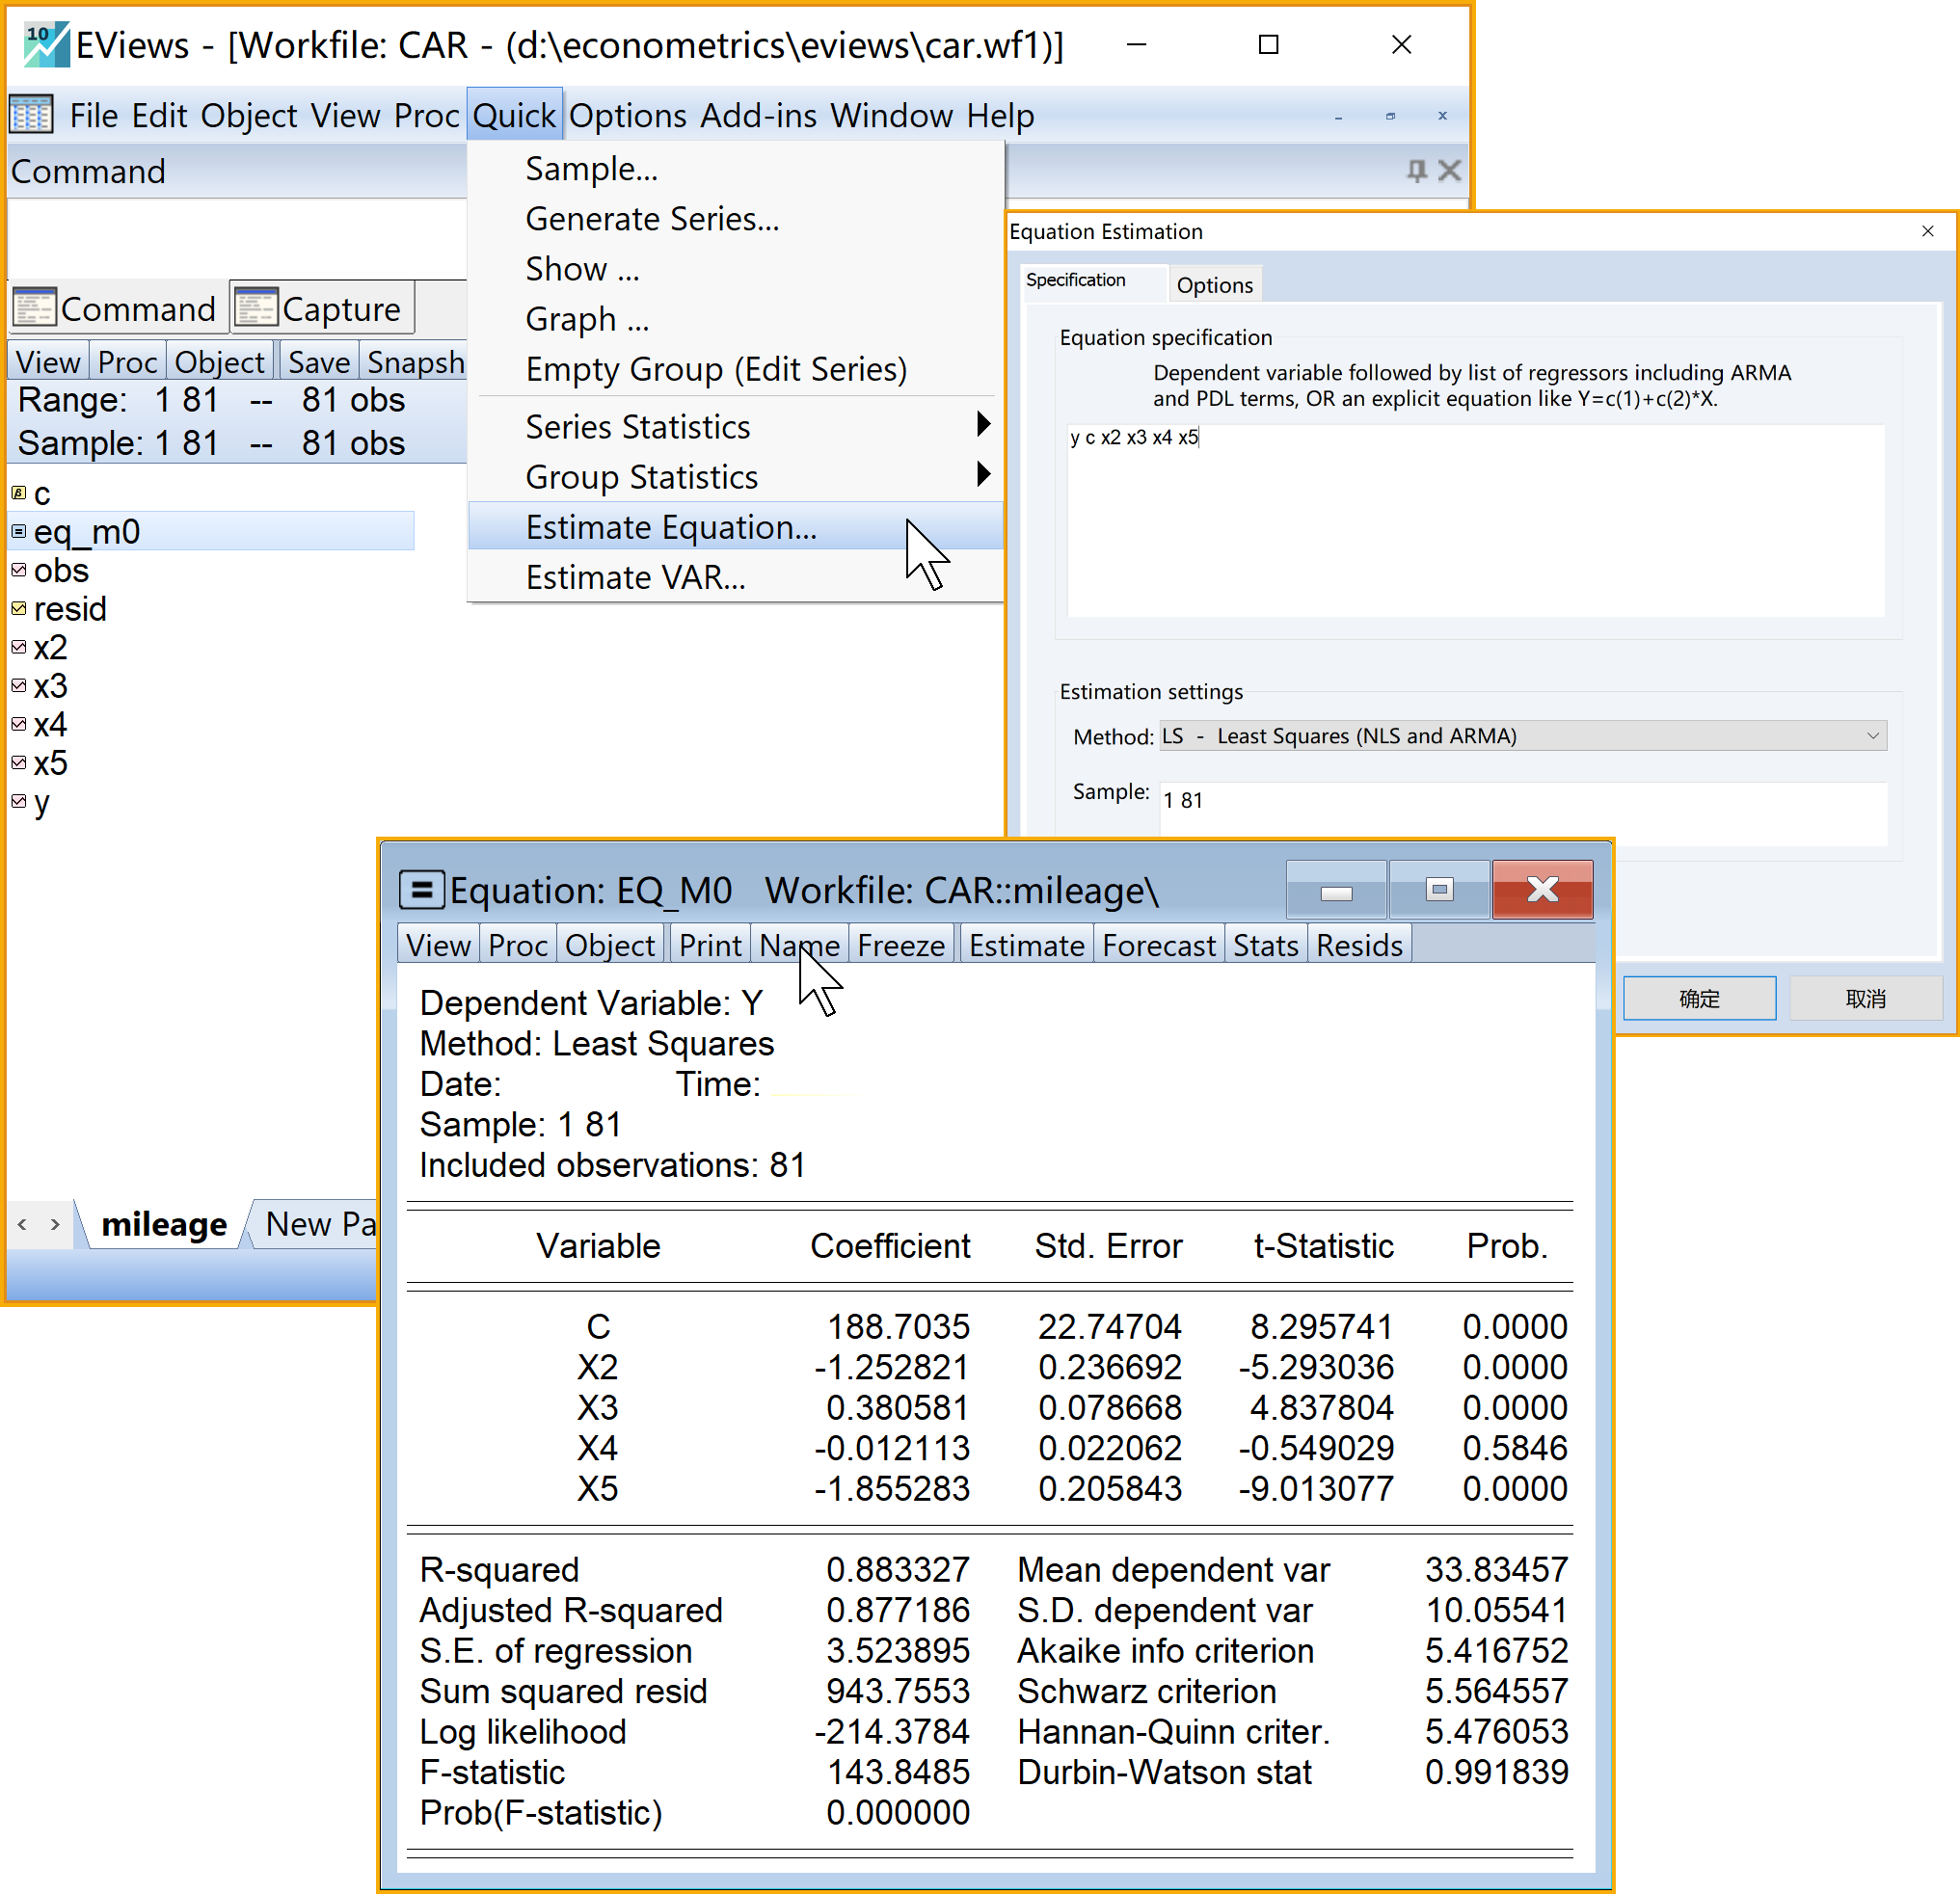
\includegraphics[width=28.24in]{picture/lab6-heteroskedasticity/2-eq-m0} 

}

\caption{主回归模型Eviews操作}\label{fig:fig-eq-m0}
\end{figure}

\begin{figure}

{\centering 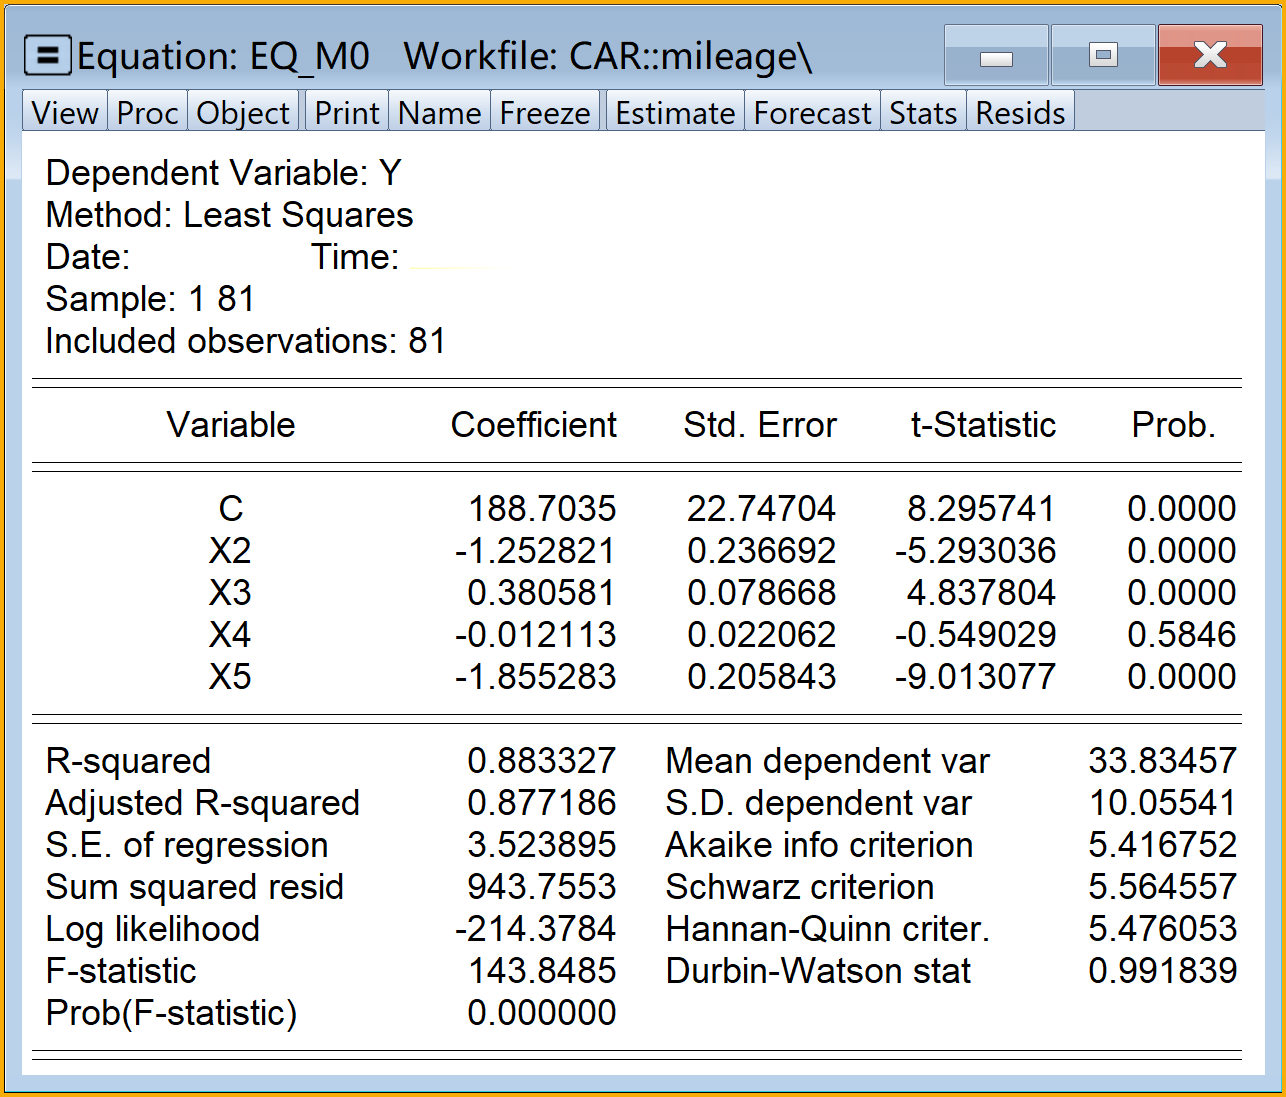
\includegraphics[width=17.86in]{picture/lab6-heteroskedasticity/2-eq-m0-report} 

}

\caption{主回归模型Eviews报告}\label{fig:fig-eq-m0-report}
\end{figure}

\subsubsection{侦查模型是否存在异方差}

\paragraph{初步观察法(观察主回归方程)}

\begin{itemize}
\tightlist
\item
  目标:观察主回归方程分析报告,分析回归报告结果,得出初步结论
\item
  思路:观察\(t^{\ast}\)检验,判定系数\(R^2\),\(F^{\ast}\)检验的关系
\item
  提示:

  \begin{itemize}
  \tightlist
  \item
    模型使用的数据是否是截面数据
  \item
    主回归分析报告的\(R^2\)值
  \item
    模型整体\(F^{\ast}\)检验结果
  \item
    斜率系数的\(t^\ast\)检验结果
  \end{itemize}
\item
  分析结论:
  根据主回归报告(见图\ref{fig:fig-eq-m0-report}),表明模型可能存在\textbf{严重}的异方差问题。
\end{itemize}

\paragraph{非正式检验法(图示法)}

\begin{itemize}
\tightlist
\item
  目标:观察\(e_i\)或\(e^2_i\)的图形模式
\item
  思路:判定\(e_i\)或\(e^2_i\)与\(i\)、\(X_i\)、\(X^2_i\)、\(Y_i\)、\(Y^2_i\)等的图形关系
\item
  提示:

  \begin{itemize}
  \tightlist
  \item
    描点图(dot
    plot)是分析一个变量的图形模式。例如\(e_i\)或\(e^2_i\)(做纵轴)相对于\(i\)(做横轴)的图形关系
  \item
    散点图(scatter
    plot)是分析两个变量之间的图形模式。例如\(e_i\)或\(e^2_i\)(做纵轴),相对于\(X_i\)或\(X^2_i\)或\(Y_i\)或\(Y^2_i\)的图形关系。
  \end{itemize}
\item
  Eviews菜单操作:

  \begin{enumerate}
  \def\labelenumi{\arabic{enumi})}
  \tightlist
  \item
    分别生成新序列\(e_i\)、\(e^2_i\)、\(Y^2_i\)和\(X^2_i\)(见图\ref{fig:fig-gen-series})

    \begin{enumerate}
    \def\labelenumii{\alph{enumii}.}
    \tightlist
    \item
      生成残差\(e^2_i\)和\(e^2_i\)序列(建议分别命名为ei和ei\_sqr)

      \begin{itemize}
      \tightlist
      \item
        命令视窗(Command)输入命令 :\texttt{series\ ei=resid}
      \item
        命令视窗(Command)输入命令
        :\texttt{series\ ei\_sqr=resid\^{}2}
      \item
        运行命令:命令行中按Enter键\\
      \end{itemize}
    \item
      生成残差\(Y^2_i\)序列(建议命名为Y\_sqr)

      \begin{itemize}
      \tightlist
      \item
        命令视窗(Command)输入命令 :\texttt{series\ Y\_sqr=Y\^{}2}
      \item
        运行命令:命令行中按Enter键\\
      \end{itemize}
    \item
      生成残差\(X^2_i\)序列(建议分别命名为X2\_sqr,X3\_sqr,X4\_sqr,X5\_sqr)

      \begin{itemize}
      \tightlist
      \item
        命令视窗(Command)输入命令 :\texttt{series\ X2\_sqr=X2\^{}2}
      \item
        命令视窗(Command)输入命令 :\texttt{series\ X3\_sqr=X3\^{}2}
      \item
        命令视窗(Command)输入命令 :\texttt{series\ X4\_sqr=X4\^{}2}
      \item
        命令视窗(Command)输入命令 :\texttt{series\ X5\_sqr=X5\^{}2}
      \item
        运行命令:上述命令行中依次按Enter键
      \end{itemize}
    \item
      查看结果:

      \begin{itemize}
      \tightlist
      \item
        双击
\includegraphics{picture/object/Series.png}\texttt{ei}
      \item
        双击
\includegraphics{picture/object/Series.png}\texttt{ei\_sqr}
      \item
        双击
\includegraphics{picture/object/Series.png}\texttt{Y\_sqr}
      \item
        双击
\includegraphics{picture/object/Series.png}\texttt{X2\_sqr}
      \item
        双击
\includegraphics{picture/object/Series.png}\texttt{X3\_sqr}
      \item
        双击
\includegraphics{picture/object/Series.png}\texttt{X4\_sqr}
      \item
        双击
\includegraphics{picture/object/Series.png}\texttt{X5\_sqr}
      \end{itemize}
    \end{enumerate}
  \item
    绘制\(e_i\)和\(e^2_i\)序列的描点图(dot
    plot)(见图\ref{fig:fig-dot-resid})

    \begin{enumerate}
    \def\labelenumii{\alph{enumii}.}
    \tightlist
    \item
      选择序列对象:键盘Ctrl键+依次单击选择序列
\includegraphics{picture/object/Series.png}\texttt{ei}和
\includegraphics{picture/object/Series.png}\texttt{ei\_sqr}
    \item
      进入引导菜单:\(\Rightarrow\) Quick \(\Rightarrow\) Graph

      \begin{itemize}
      \tightlist
      \item
        选择绘图类型(Graph type):Dot plot
      \item
        选择绘图细节(Detail):\(\Rightarrow\) Multiple series
        \(\Rightarrow\) 下拉选择 Multiple graphs
      \end{itemize}
    \item
      点击完成:OK
    \item
      命名并保存绘图(graph)对象
\includegraphics{picture/object/Graph.png}:建议命名为dot\_resid
    \item
      查看结果:双击
\includegraphics{picture/object/Graph.png}dot\_resid(见图\ref{fig:fig-dot-resid-report})
    \end{enumerate}
  \item
    绘制\(e_i\)序列对\(Y_i\);
    \(X_{1 i};X_{2 i};X_{3 i};X_{4 i}\)的散点图图(scatter
    plot)(见图\ref{fig:fig-scatter-ei})

    \begin{enumerate}
    \def\labelenumii{\alph{enumii}.}
    \tightlist
    \item
      选择序列对象:键盘Ctrl键+依次单击选择序列
\includegraphics{picture/object/Series.png}ei;
\includegraphics{picture/object/Series.png}Y;
\includegraphics{picture/object/Series.png}X2;
\includegraphics{picture/object/Series.png}X3;
\includegraphics{picture/object/Series.png}X4;
\includegraphics{picture/object/Series.png}X5
    \item
      进入引导菜单:\(\Rightarrow\) Quick \(\Rightarrow\) Graph

      \begin{itemize}
      \tightlist
      \item
        选择绘图类型(Graph type):Scatter
      \item
        选择绘图细节(Detail):\(\Rightarrow\) Multiple series
        \(\Rightarrow\) 下拉选择 Multiple graphs - First vs.~all
      \end{itemize}
    \item
      点击完成:OK
    \item
      命名并保存绘图(graph)对象
\includegraphics{picture/object/Graph.png}:建议命名为scatter\_ei
    \item
      查看结果:双击
\includegraphics{picture/object/Graph.png}scatter\_ei(见图\ref{fig:fig-scatter-ei})
    \end{enumerate}
  \item
    绘制\(e^2_i\)序列对\(Y_i\);
    \(X_{1 i};X_{2 i};X_{3 i};X_{4 i}\)的散点图图(scatter
    plot)(见图\ref{fig:fig-scatter-ei-sqr})

    \begin{enumerate}
    \def\labelenumii{\alph{enumii}.}
    \tightlist
    \item
      选择序列对象:键盘Ctrl键+依次单击选择序列
\includegraphics{picture/object/Series.png}ei\_sqr;
\includegraphics{picture/object/Series.png}Y;
\includegraphics{picture/object/Series.png}X2;
\includegraphics{picture/object/Series.png}X3;
\includegraphics{picture/object/Series.png}X4;
\includegraphics{picture/object/Series.png}X5
    \item
      进入引导菜单:\(\Rightarrow\) Quick \(\Rightarrow\) Graph

      \begin{itemize}
      \tightlist
      \item
        选择绘图类型(Graph type):Scatter
      \item
        选择绘图细节(Detail):\(\Rightarrow\) Multiple series
        \(\Rightarrow\) 下拉选择 Multiple graphs - First vs.~all
      \end{itemize}
    \item
      点击完成:OK
    \item
      命名并保存绘图(graph)对象
\includegraphics{picture/object/Graph.png}:建议命名为scatter\_ei\_sqr
    \item
      查看结果:双击
\includegraphics{picture/object/Graph.png}scatter\_ei\_sqr(见图\ref{fig:fig-scatter-ei-sqr})
    \end{enumerate}
  \end{enumerate}
\end{itemize}

\begin{figure}

{\centering 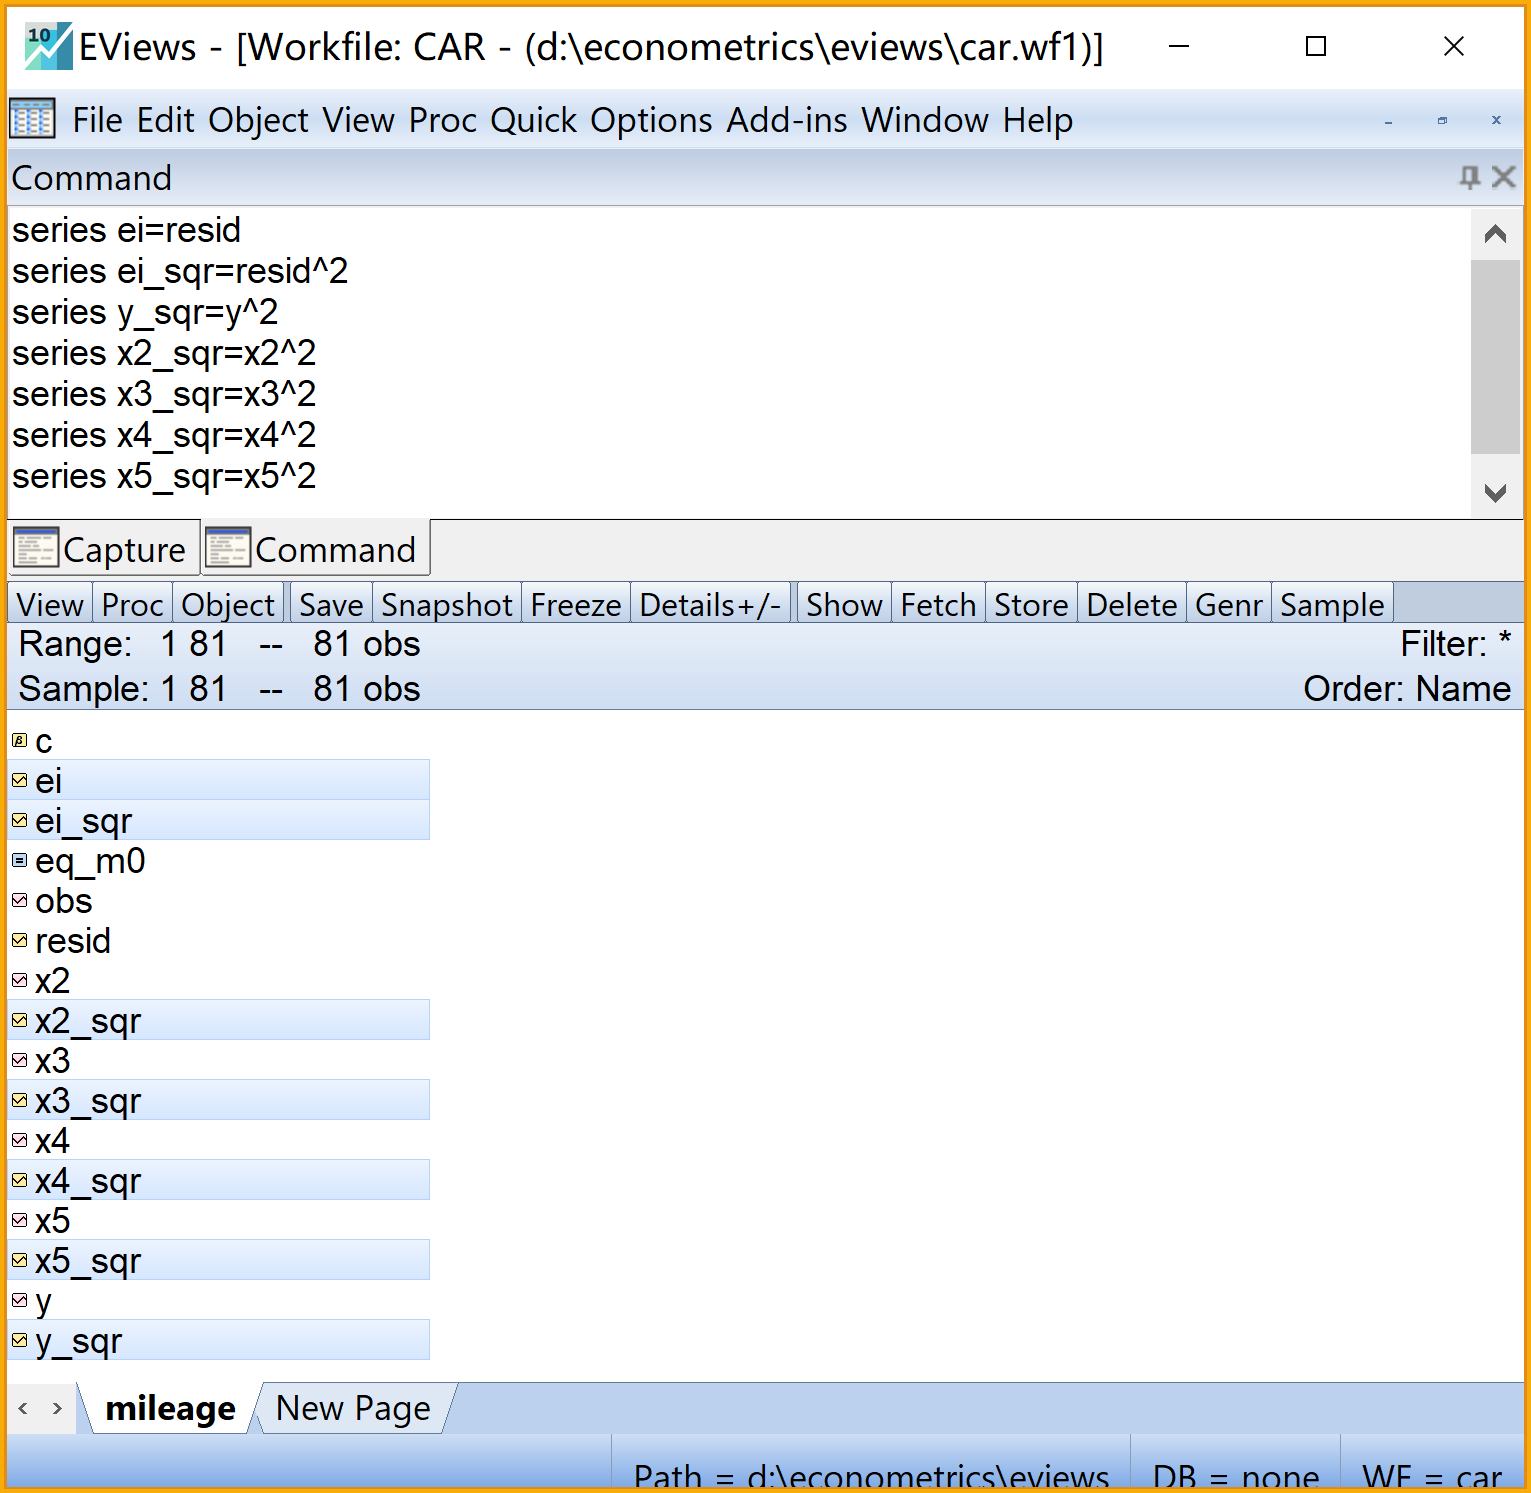
\includegraphics[width=21.26in]{picture/lab6-heteroskedasticity/3-generate-series} 

}

\caption{生成相关变量}\label{fig:fig-gen-series}
\end{figure}

\begin{figure}

{\centering 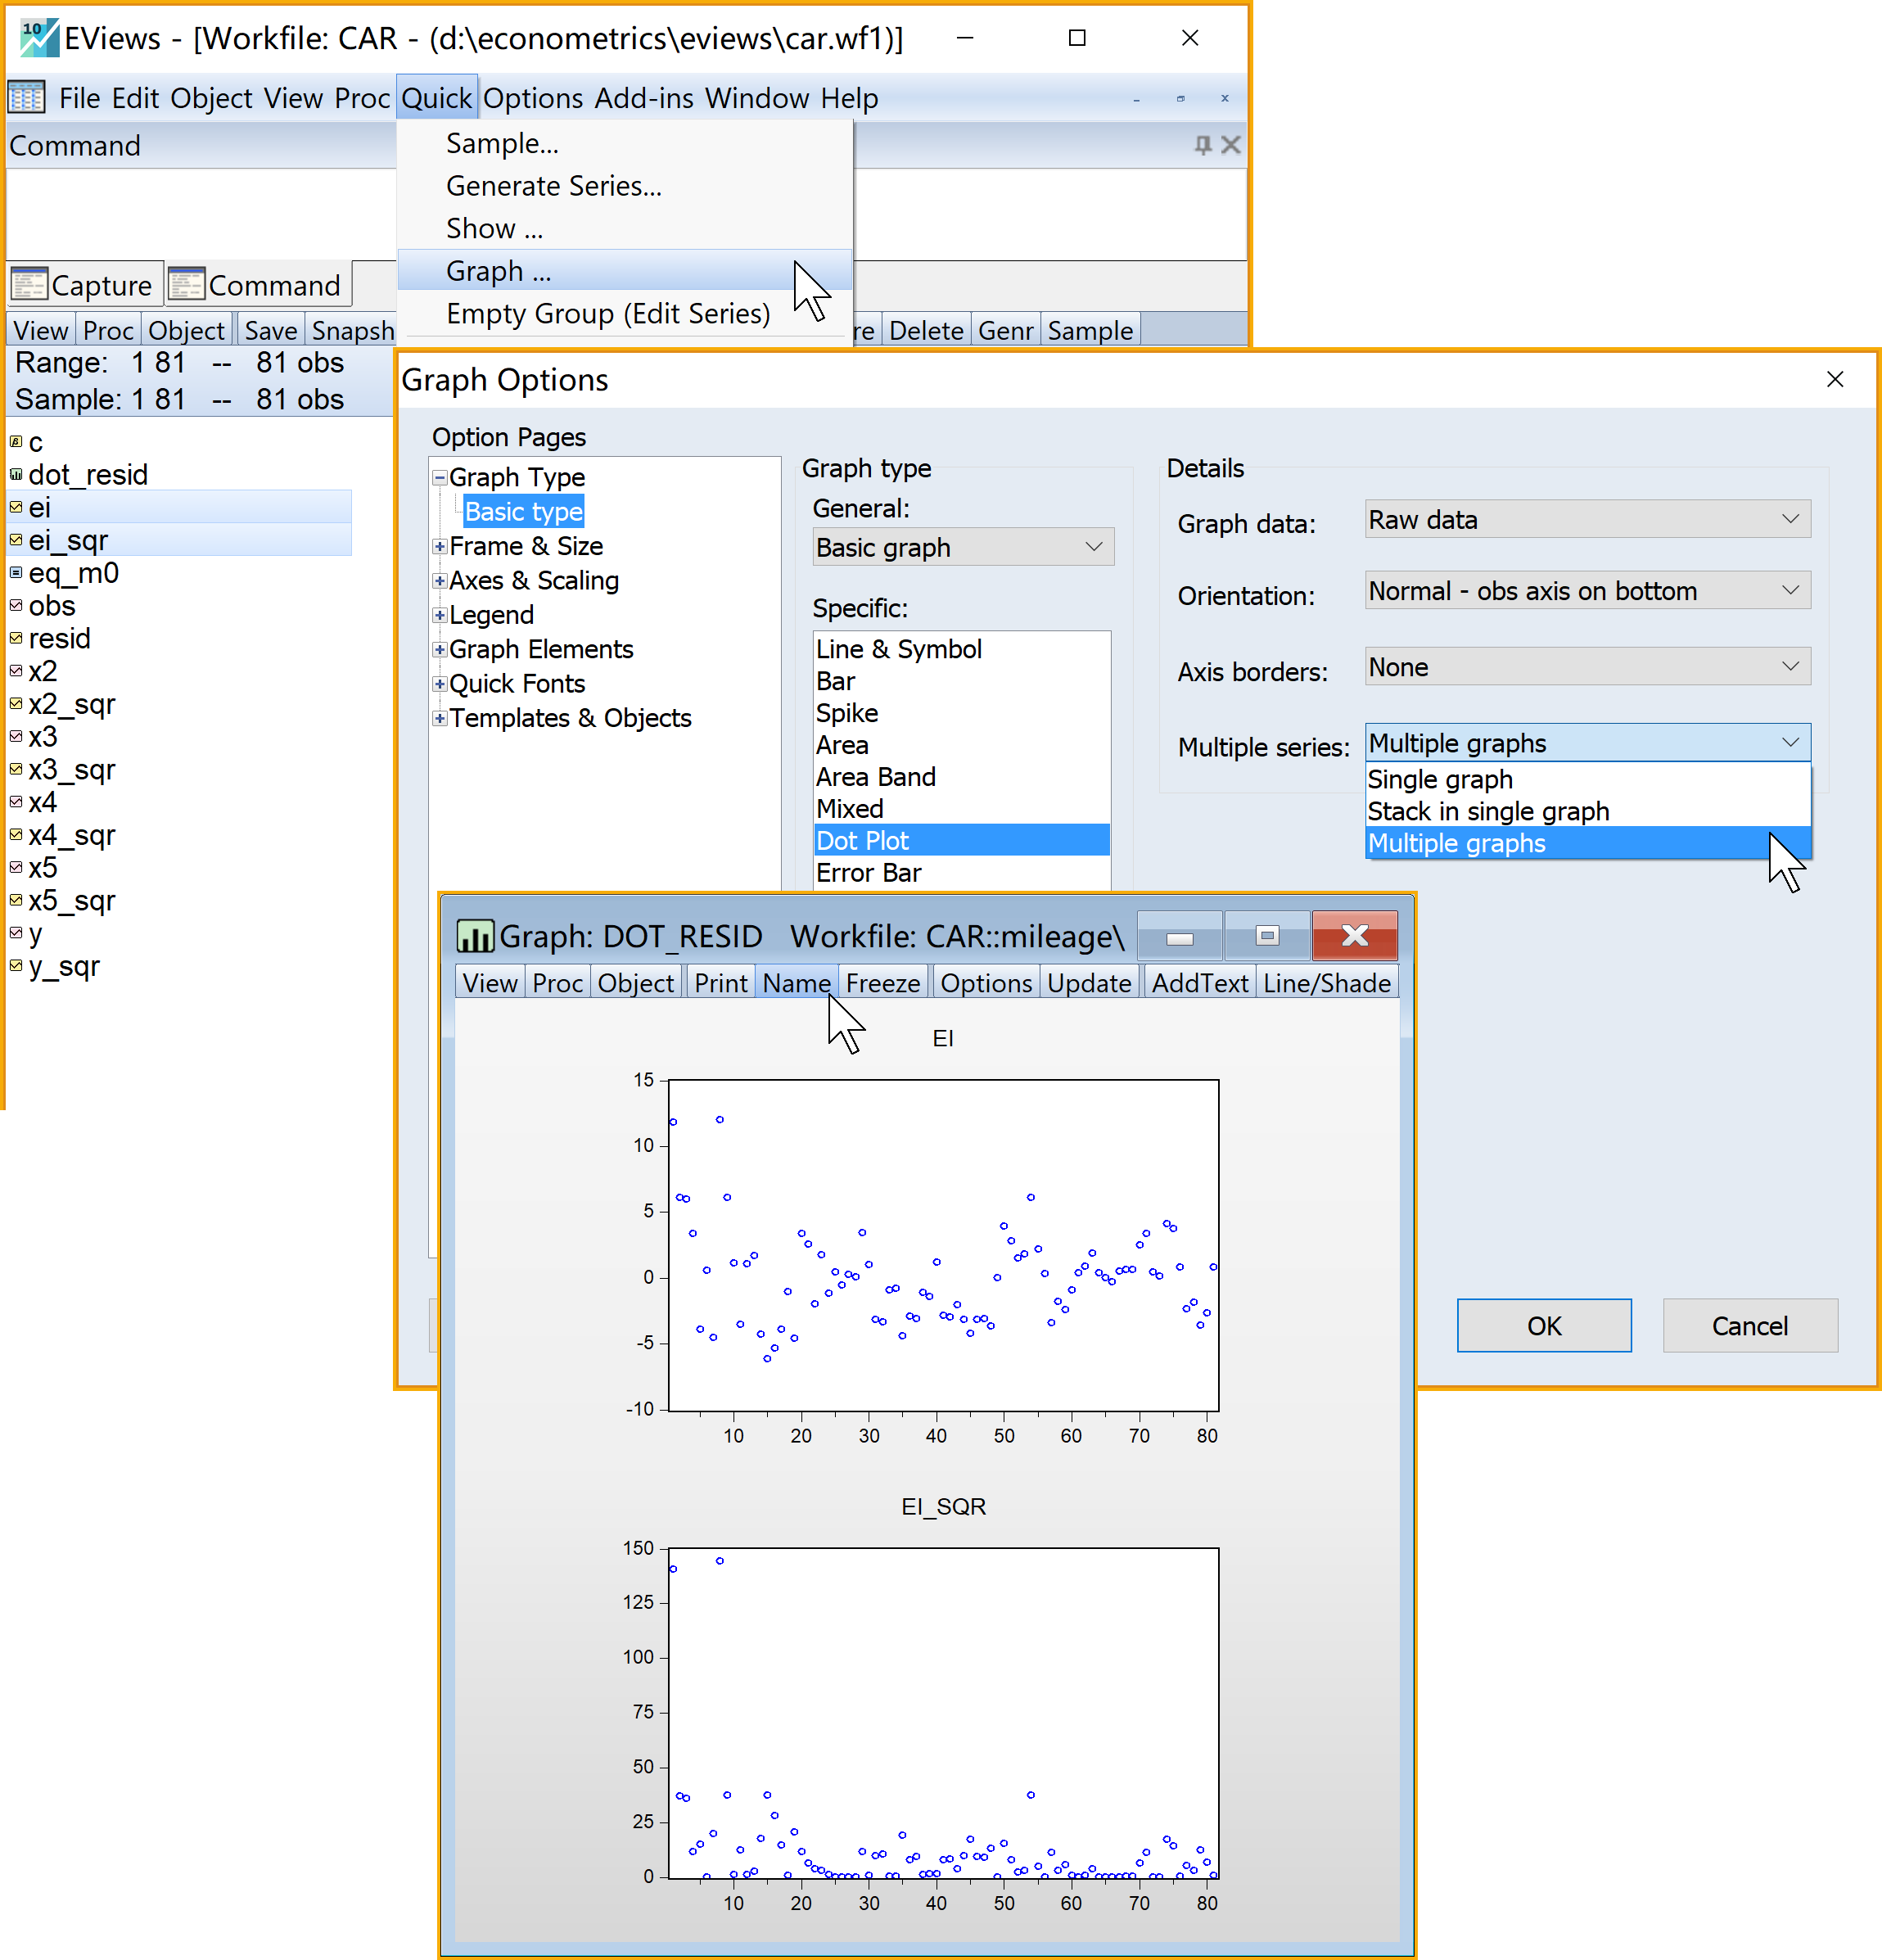
\includegraphics[width=31.93in]{picture/lab6-heteroskedasticity/3-dot-resid} 

}

\caption{残差及残差平方的描点图}\label{fig:fig-dot-resid}
\end{figure}

\begin{figure}

{\centering 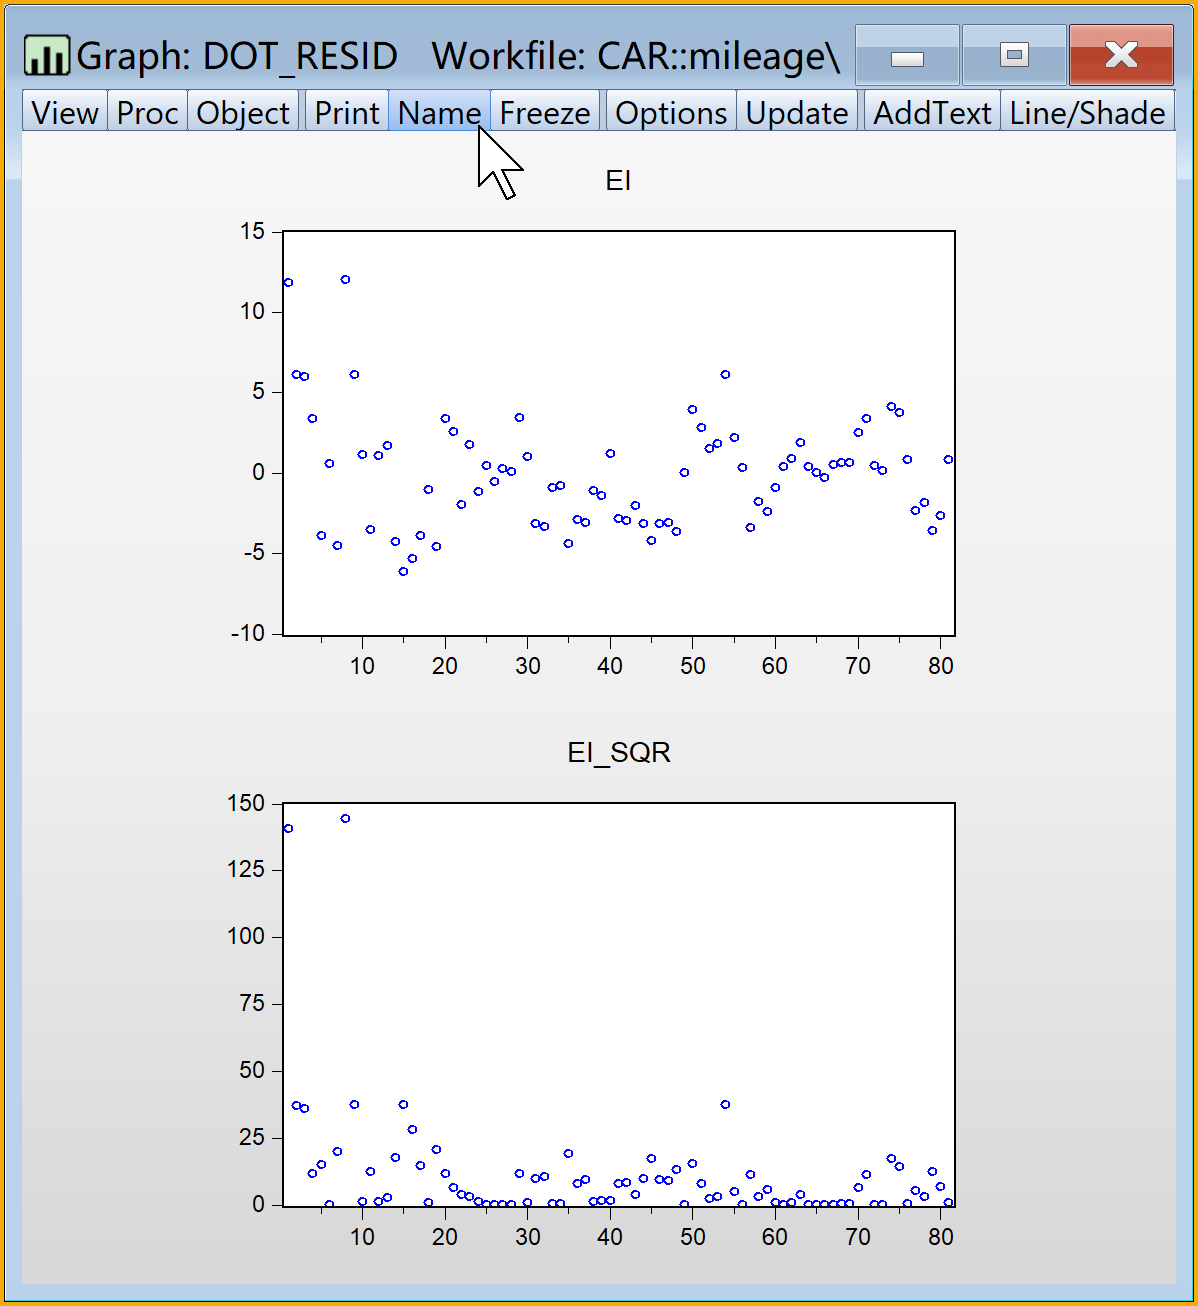
\includegraphics[width=16.64in]{picture/lab6-heteroskedasticity/3-dot-resid-report} 

}

\caption{残差及残差平方的描点图报告}\label{fig:fig-dot-resid-report}
\end{figure}

\begin{figure}

{\centering 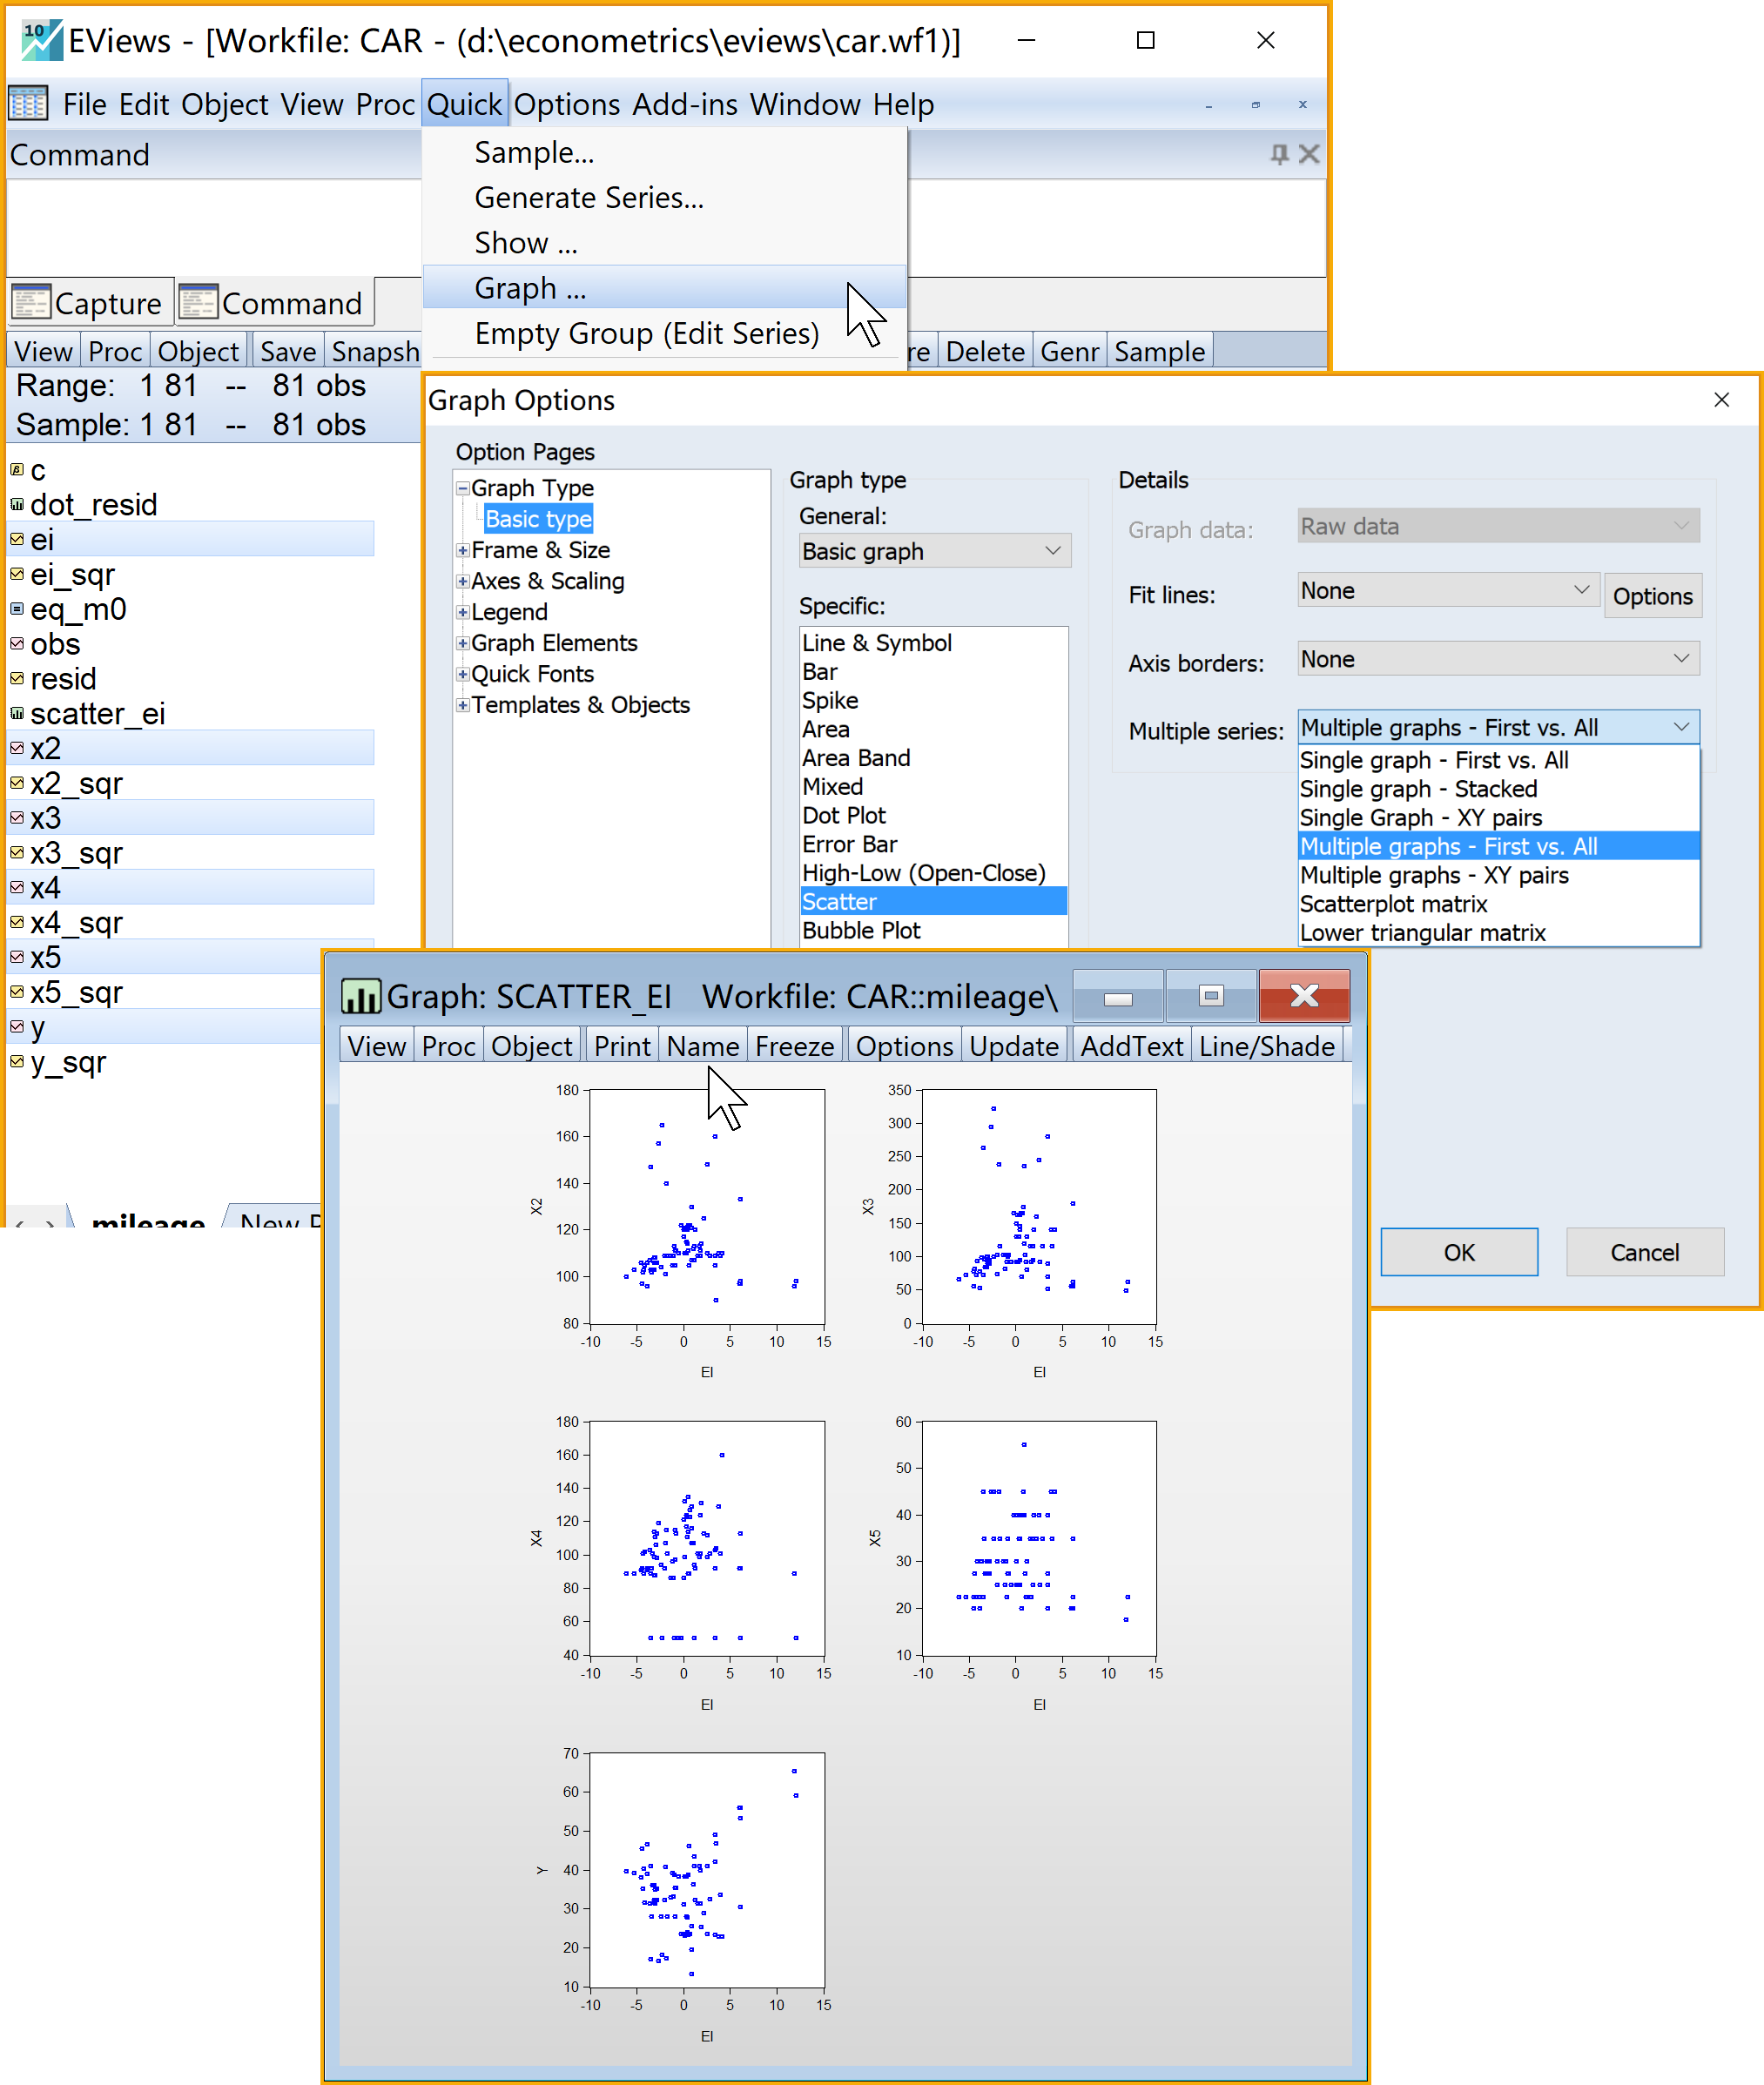
\includegraphics[width=28.14in]{picture/lab6-heteroskedasticity/3-scatter-ei} 

}

\caption{残差与模型变量的散点图}\label{fig:fig-scatter-ei}
\end{figure}

\begin{figure}

{\centering 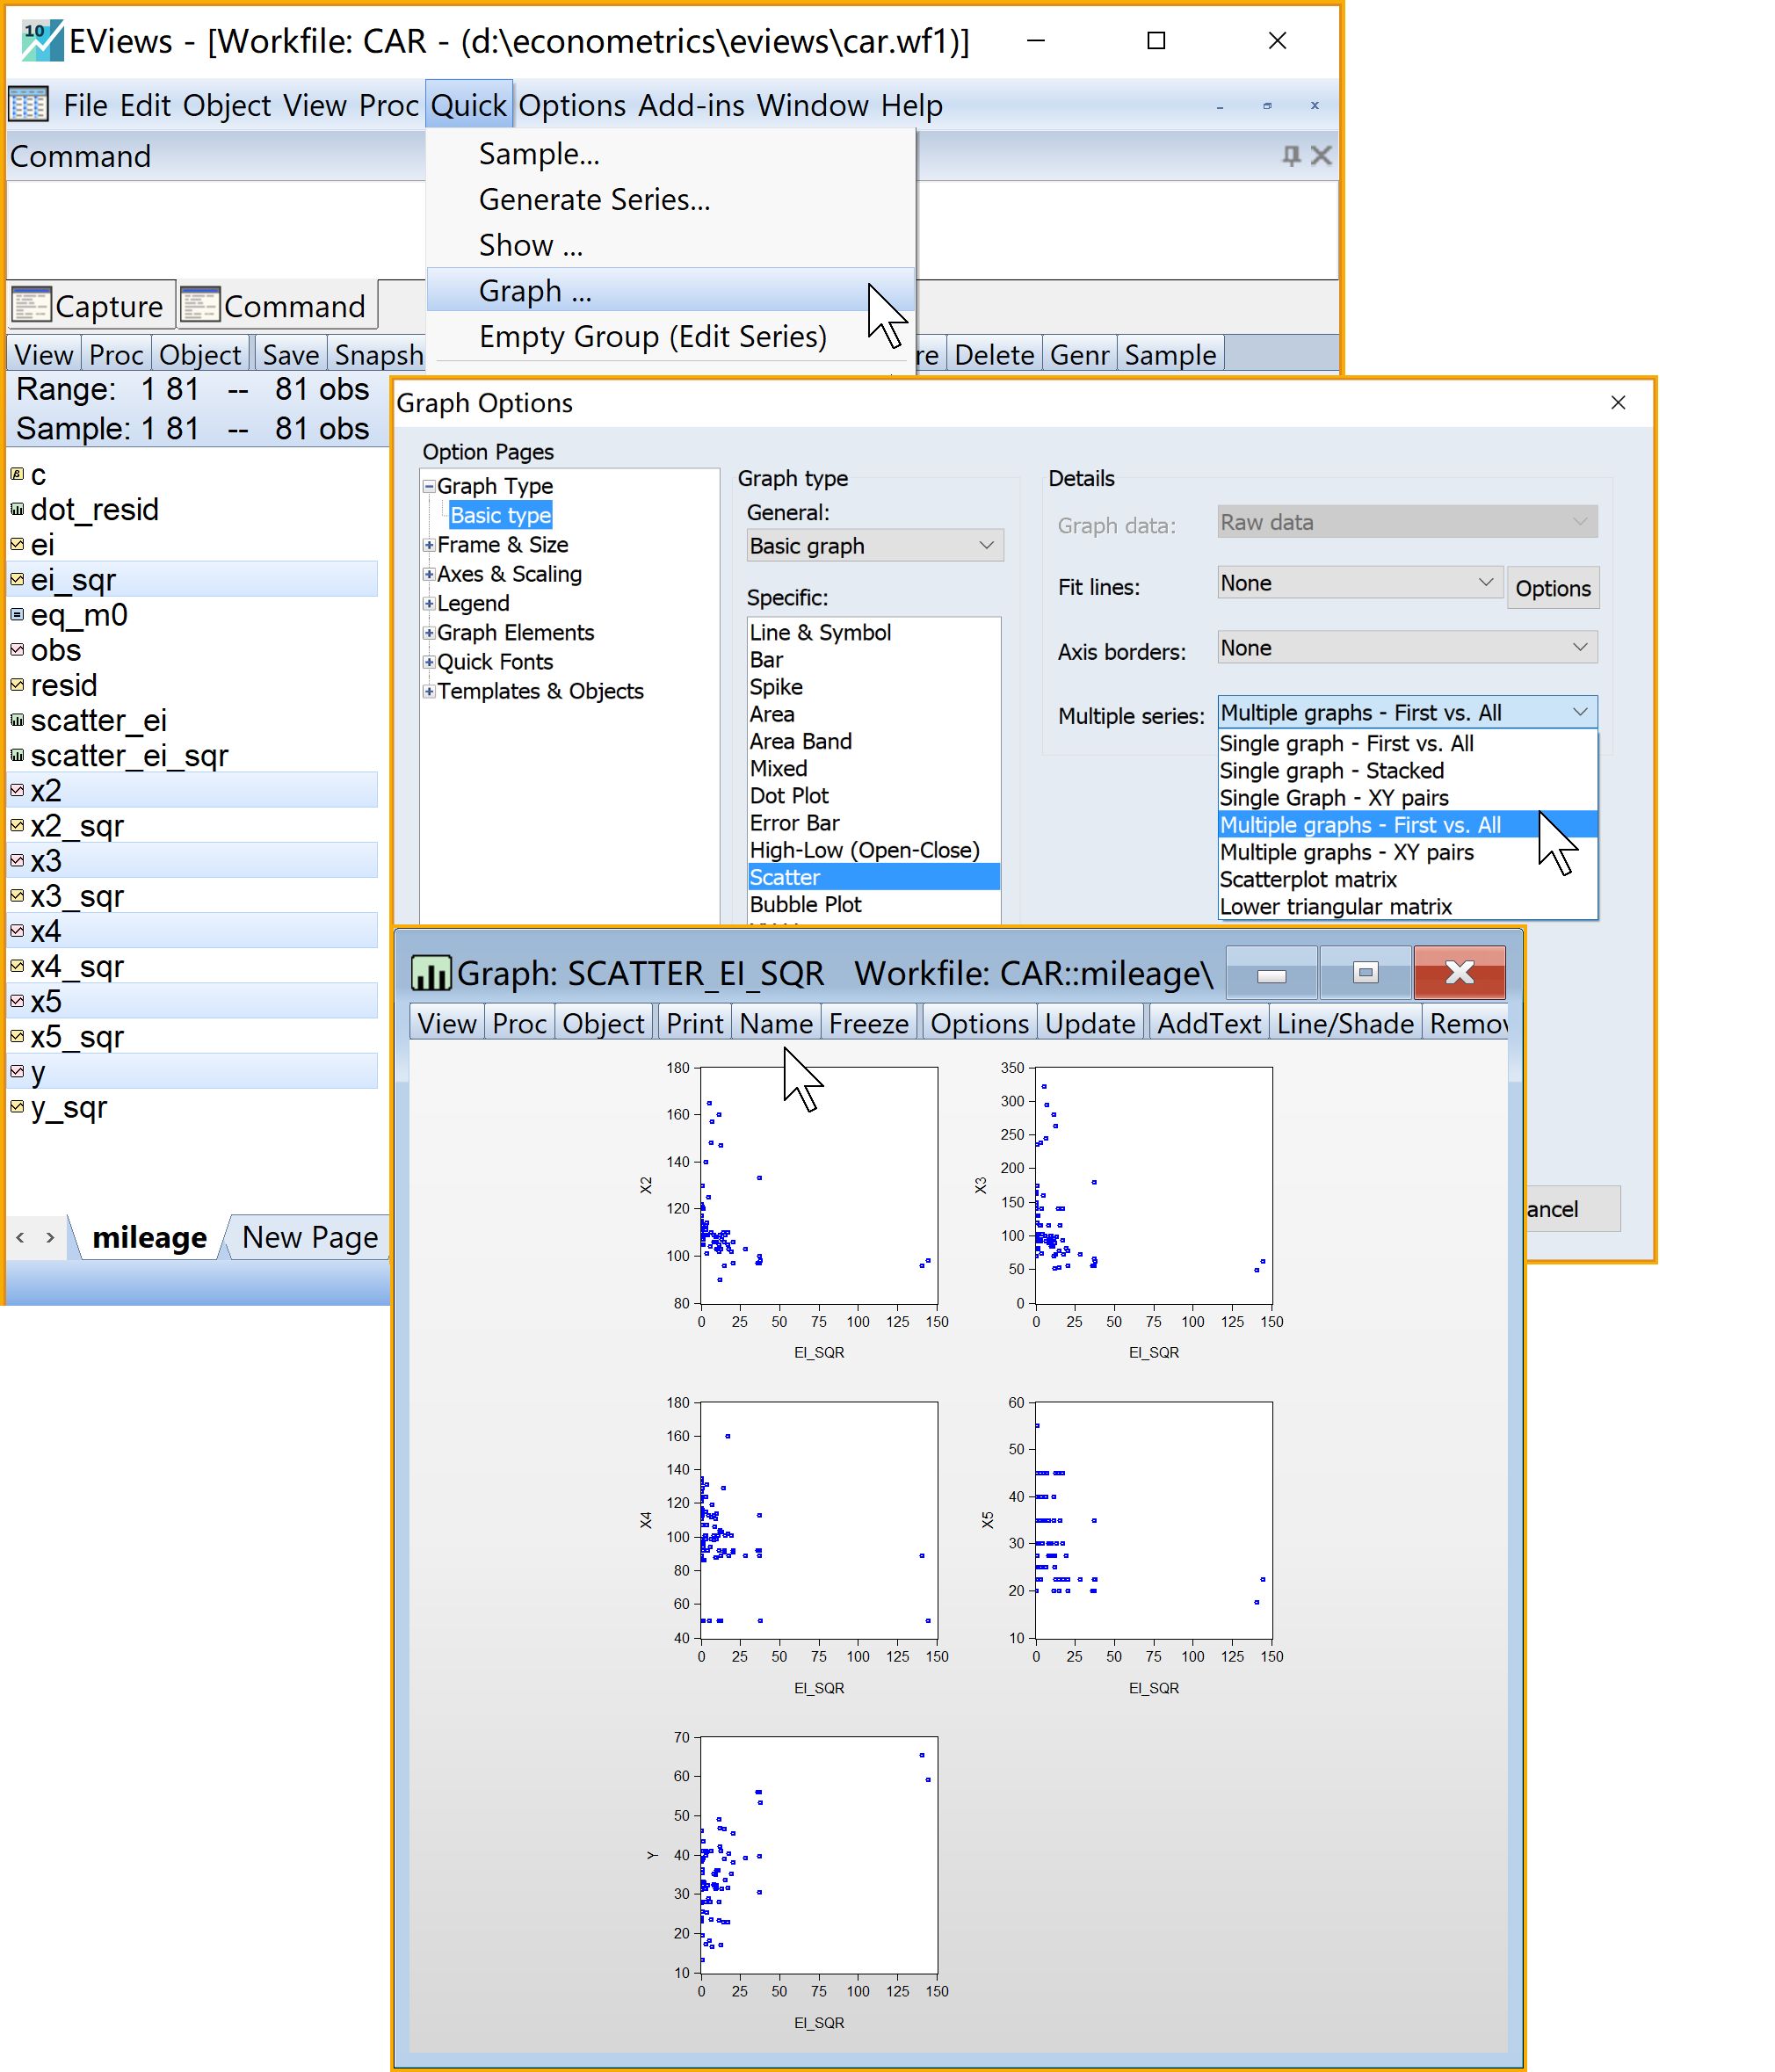
\includegraphics[width=28.06in]{picture/lab6-heteroskedasticity/3-scatter-ei-sqr} 

}

\caption{残差平方与模型变量的散点图}\label{fig:fig-scatter-ei-sqr}
\end{figure}

\paragraph{正式检验法}

\begin{itemize}
\item
  目标:利用Eviews的异方差诊断菜单,分别对主回归模型\eqref{eq:M0-car}进行
  进行异方差诊断。
\item
  思路:诊断方法包括Park检验、Glejser检验、BPG检验和White检验等。根据辅助诊断方程的理论假设,分析Eviews诊断报告,与相关参考标准进行比较,得到相关结论
\item
  定义:

  \begin{itemize}
  \tightlist
  \item
    主回归模型(Main
    Model)是指Y变量对全部X变量的线性回归(如主模型\eqref{eq:M0-car})
  \item
    辅助诊断模型(Auxiliary
    Model)是指利用主回归模型的残差序列\(e_i\)对X变量进行特定的线性回归(具体的辅助诊断模型有多个)
  \end{itemize}
\item
  提示:

  \begin{itemize}
  \tightlist
  \item
    操作提示:用Eviews的异方差诊断菜单 \(\Rightarrow\) View
    \(\Rightarrow\) Residual Diagnostics \(\Rightarrow\)
    Heteroskedasticity Test
  \item
    诊断提示:若发现假设检验结果不显著(视具体检验方法而不同)则表明主模型\eqref{eq:M0-car}为同方差;否则就表明主模型\eqref{eq:M0-car}为异方差
  \item
    理论提示:你也可以自己根据实际情况设定个性化的辅助诊断方程
  \end{itemize}
\end{itemize}

\hypertarget{park}{%
\subparagraph{Park检验法}\label{park}}

\begin{itemize}
\tightlist
\item
  诊断辅助方程:
\end{itemize}

\begin{equation}
ln(e^2_i)=\hat{\alpha}_1+\hat{\alpha}_2ln(X_{2i})+\cdots+\hat{\alpha}_kln(X_{ki})+v_i \label{eq:A-park}
\end{equation}

\begin{itemize}
\item
  诊断标准:

  \begin{itemize}
  \tightlist
  \item
    如果诊断辅助方程\eqref{eq:A-park}的F检验\textbf{不显著}(对应的概率值P\textgreater{}0.1),则表明主模型\eqref{eq:M0-car}是同方差
  \item
    如果诊断辅助方程\eqref{eq:A-park}的F检验\textbf{显著}(对应的概率值P\textless{}0.1),则表明主模型\eqref{eq:M0-car}是异方差。
  \end{itemize}
\item
  Eviews说明:Eviews没有Park异方差检验的诊断菜单,但可以通过选择Harvey异方差菜单,并修改相关变量设置来得到Park检验报告。
\item
  Eviews操作(菜单操作实现,具体见图\ref{fig:fig-park-test}):

  \begin{enumerate}
  \def\labelenumi{\arabic{enumi})}
  \tightlist
  \item
    打开主方程:双击方程(equation)对象
\includegraphics{picture/object/Equation.png}eq\_m0\\
  \item
    进入引导菜单:\(\Rightarrow\) View \(\Rightarrow\) Residual
    Diagnostics \(\Rightarrow\) Heteroskedasticity Test \(\Rightarrow\)
    Specification

    \begin{itemize}
    \tightlist
    \item
      设置诊断方法(Test type): 点击选择Harvey
    \item
      设置诊断方程(Regressors):输入c log(X2) log(X3) log(X4)
      log(X5)\\
    \end{itemize}
  \item
    完成设置:点击Ok\\
  \item
    命名并保存表格(table)对象
\includegraphics{picture/object/Table.png}

    \begin{itemize}
    \tightlist
    \item
      另存为表格(table)对象:点击Freeze
    \item
      命名并保存表格(talbe)对象:点击name(建议为tab\_park)
    \item
      查看结果:双击
\includegraphics{picture/object/Table.png}tab\_park
    \end{itemize}
  \end{enumerate}
\end{itemize}

具体Eviews报告见\ref{fig:fig-park-report}:

\begin{figure}

{\centering 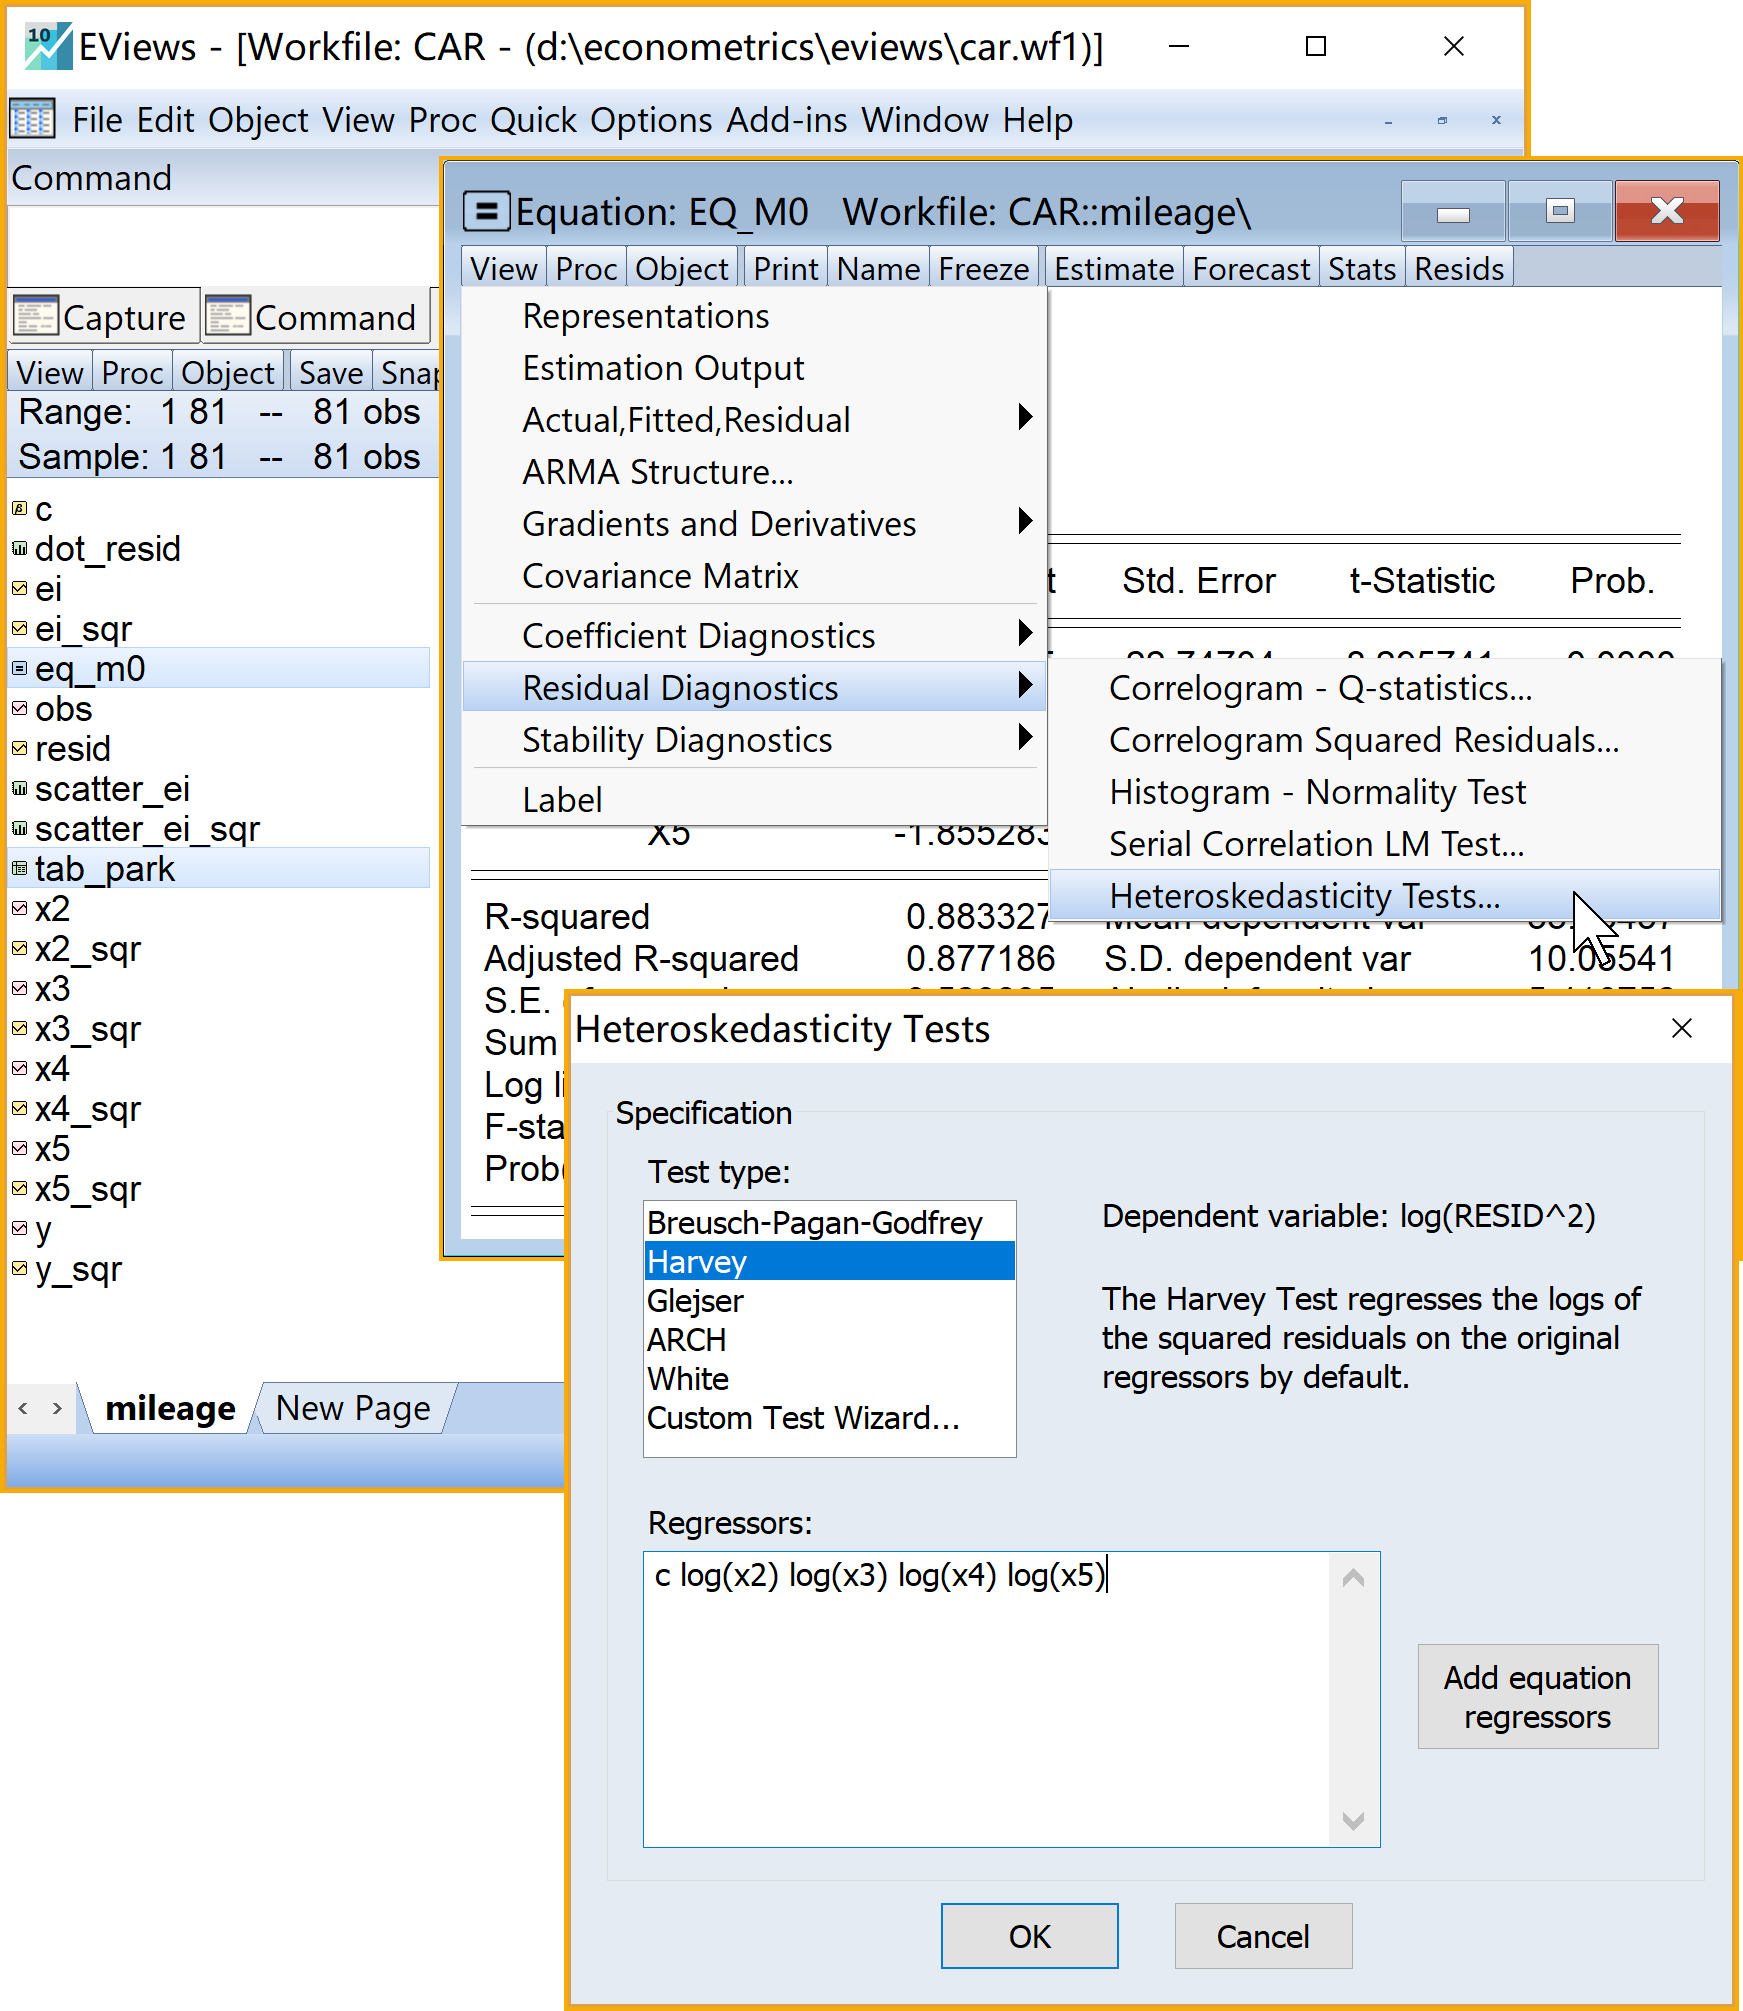
\includegraphics[width=24.21in]{picture/lab6-heteroskedasticity/4-test-park1} 

}

\caption{Park异方差检验操作}\label{fig:fig-park-test}
\end{figure}

\begin{figure}

{\centering 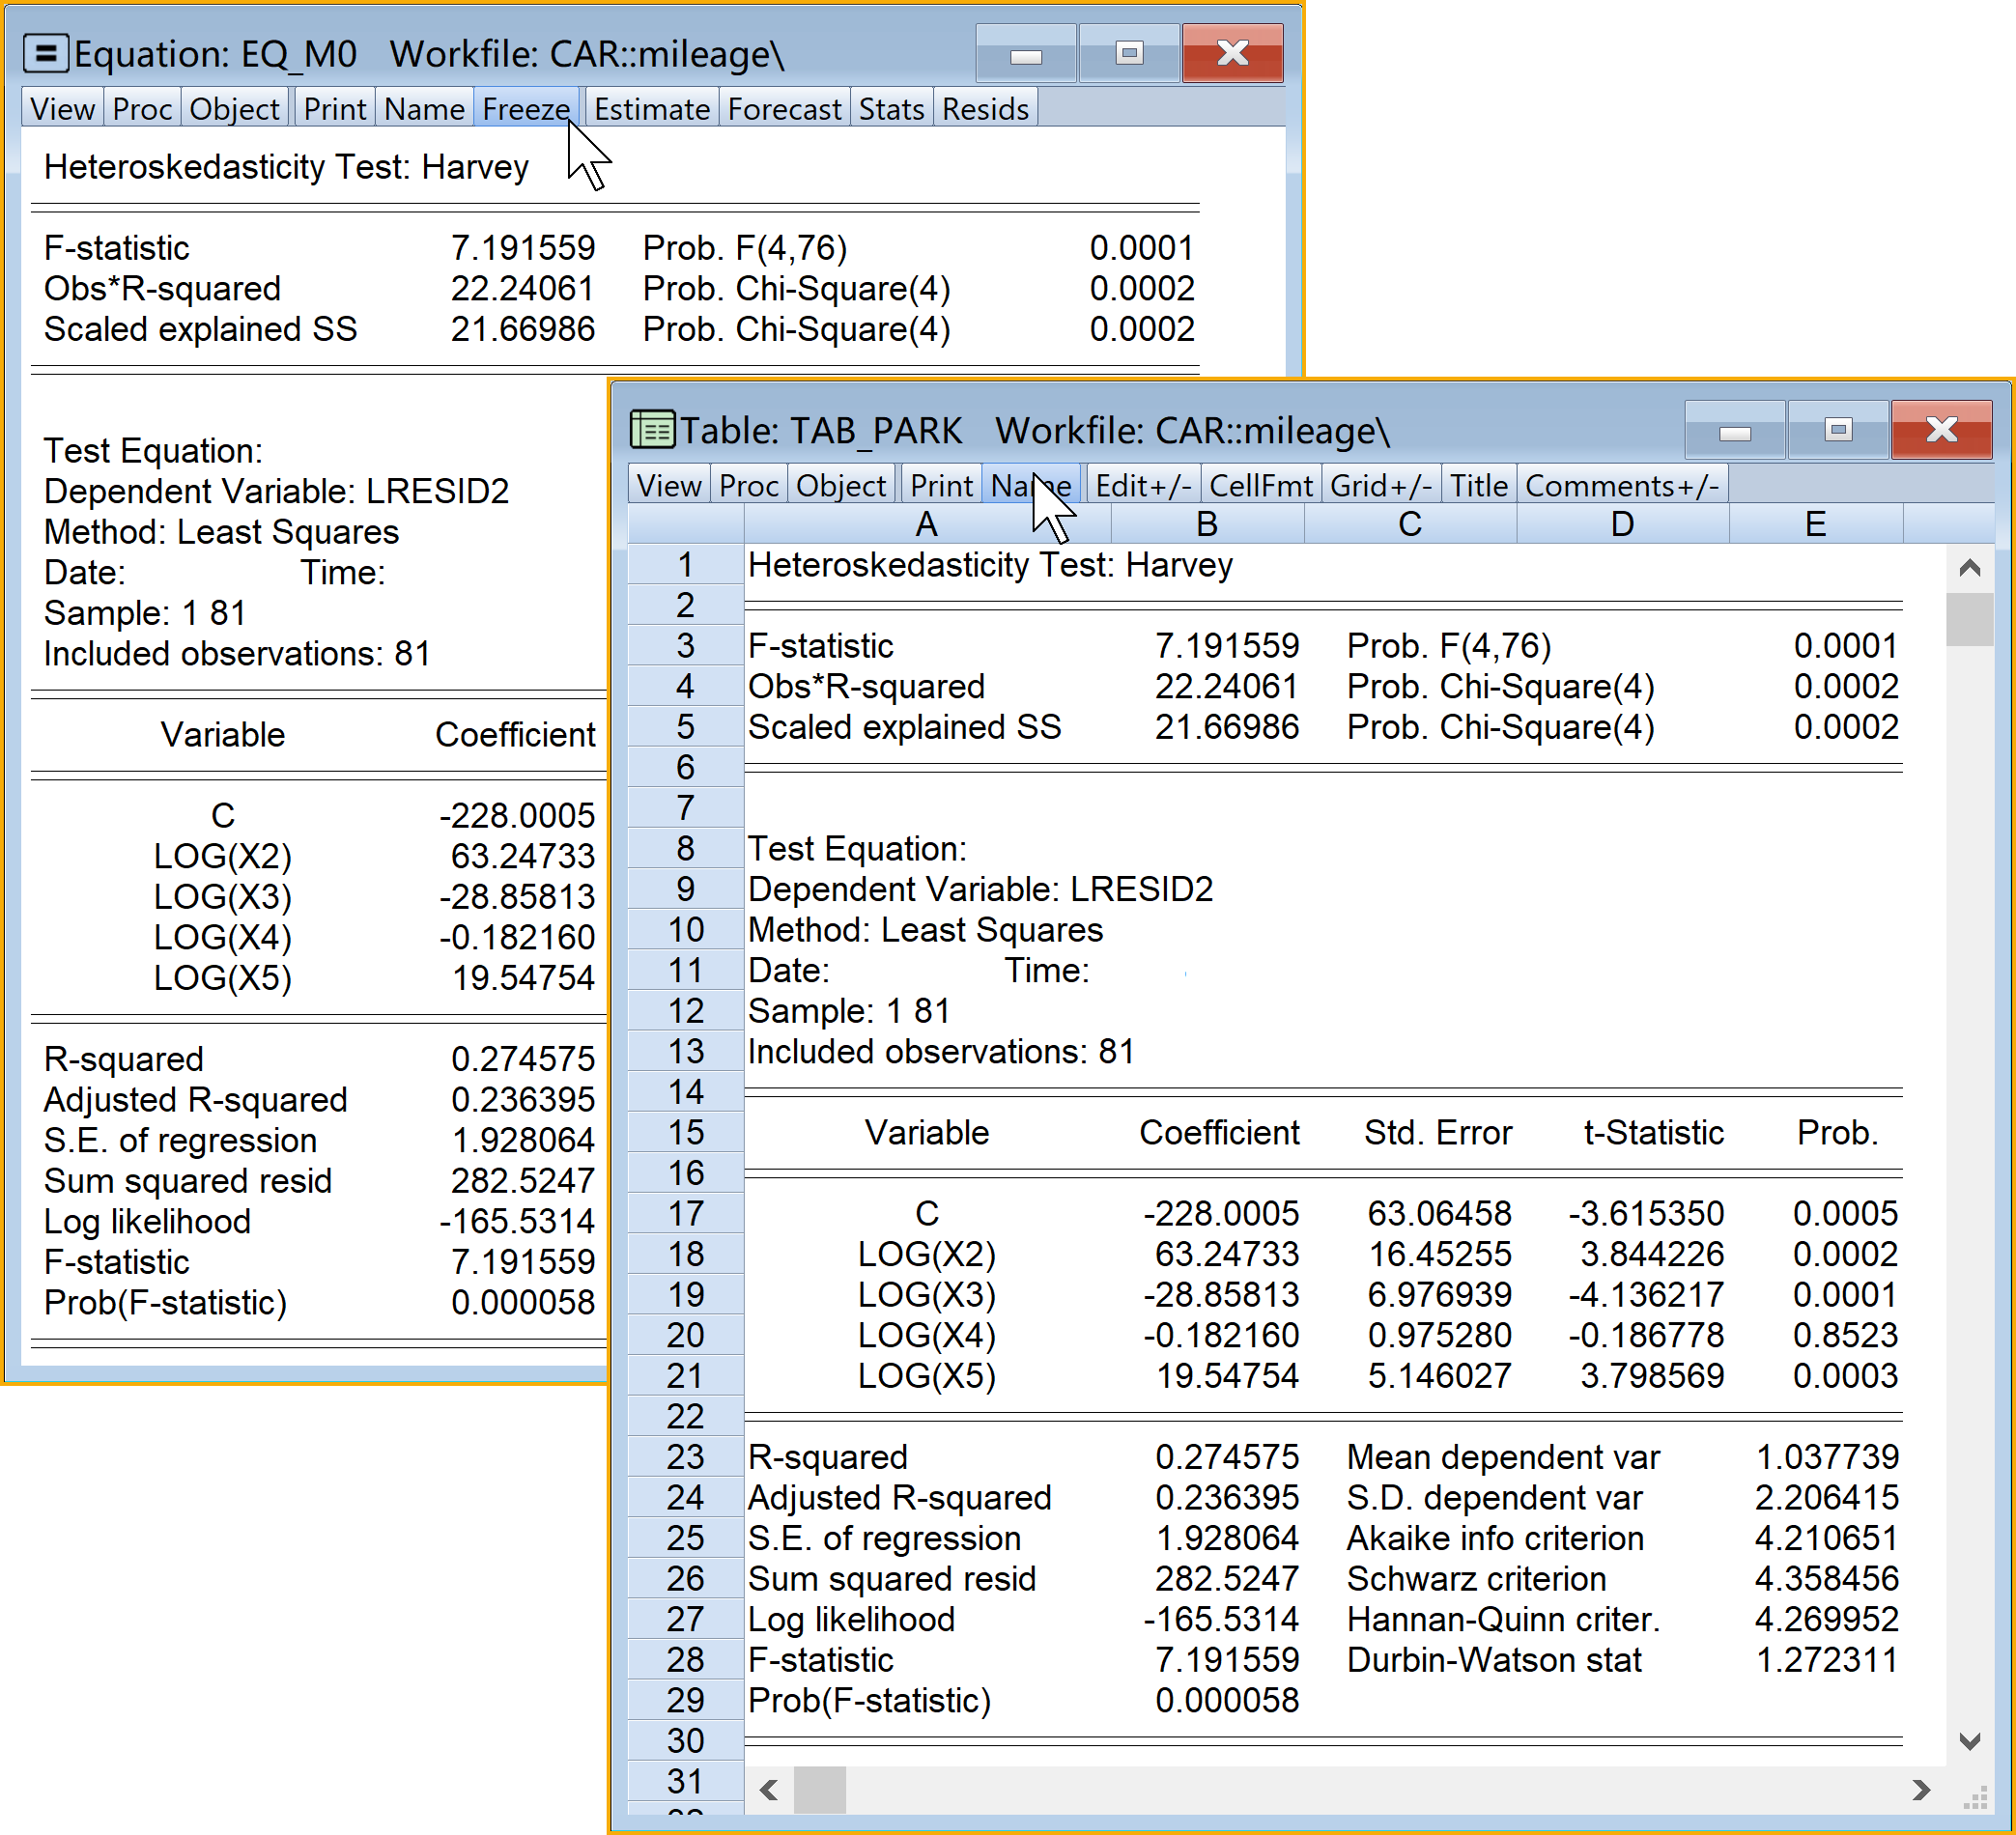
\includegraphics[width=28.99in]{picture/lab6-heteroskedasticity/4-test-park2} 

}

\caption{Park异方差检验报告}\label{fig:fig-park-report}
\end{figure}

\hypertarget{glejser}{%
\subparagraph{Glejser检验法}\label{glejser}}

\begin{itemize}
\tightlist
\item
  诊断辅助方程:
\end{itemize}

\begin{align}
|e_i| & =\hat{\alpha}_1+\hat{\alpha}_2X_{2i}+\cdots+\hat{\alpha}_kX_{ki}+v_i &&\text{G1} \label{eq:G1}\\
|e_i| & =\hat{\alpha}_1+\hat{\alpha}_2\sqrt{X_{2i}}+\cdots+\hat{\alpha}_k\sqrt{X_{ki}}+v_i &&\text{G2} \label{eq:G2}\\
|e_i| & =\hat{\alpha}_1+\hat{\alpha}_2\frac{1}{X_{2i}}+\cdots+\hat{\alpha}_k\frac{1}{X_{ki}}+v_i &&\text{G3} \label{eq:G3}
\end{align}

\begin{itemize}
\tightlist
\item
  诊断标准:

  \begin{itemize}
  \tightlist
  \item
    如果诊断辅助方程\eqref{eq:A-park}的F检验\textbf{不显著}(对应的概率值P\textgreater{}0.1),则表明主模型\eqref{eq:M0-car}是同方差
  \item
    如果诊断辅助方程\eqref{eq:A-park}的F检验\textbf{显著}(对应的概率值P\textless{}0.1),则表明主模型\eqref{eq:M0-car}是异方差。
  \end{itemize}
\item
  Eviews操作1(Glejser辅助方程\eqref{eq:G1},具体见图\ref{fig:fig-G1-test}):

  \begin{enumerate}
  \def\labelenumi{\arabic{enumi})}
  \tightlist
  \item
    打开主方程:双击方程(equation)对象
\includegraphics{picture/object/Equation.png}eq\_m0\\
  \item
    进入引导菜单:\(\Rightarrow\) View \(\Rightarrow\) Residual
    Diagnostics \(\Rightarrow\) Heteroskedasticity Test \(\Rightarrow\)
    Specification

    \begin{itemize}
    \tightlist
    \item
      设置诊断方法(Test type): 点击选择Glejser
    \item
      设置诊断方程(Regressors):输入c X2 c X3 c X4 c X5\\
    \end{itemize}
  \item
    完成设置:点击Ok\\
  \item
    命名并保存表格(table)对象
\includegraphics{picture/object/Table.png}

    \begin{itemize}
    \tightlist
    \item
      另存为表格(table)对象:点击Freeze
    \item
      命名并保存表格(table)对象:点击name(建议为tab\_G1)
    \item
      查看结果:双击
\includegraphics{picture/object/Table.png}tab\_G1
    \end{itemize}
  \end{enumerate}
\end{itemize}

具体Eviews报告见\ref{fig:fig-G1-report}:

\begin{figure}

{\centering 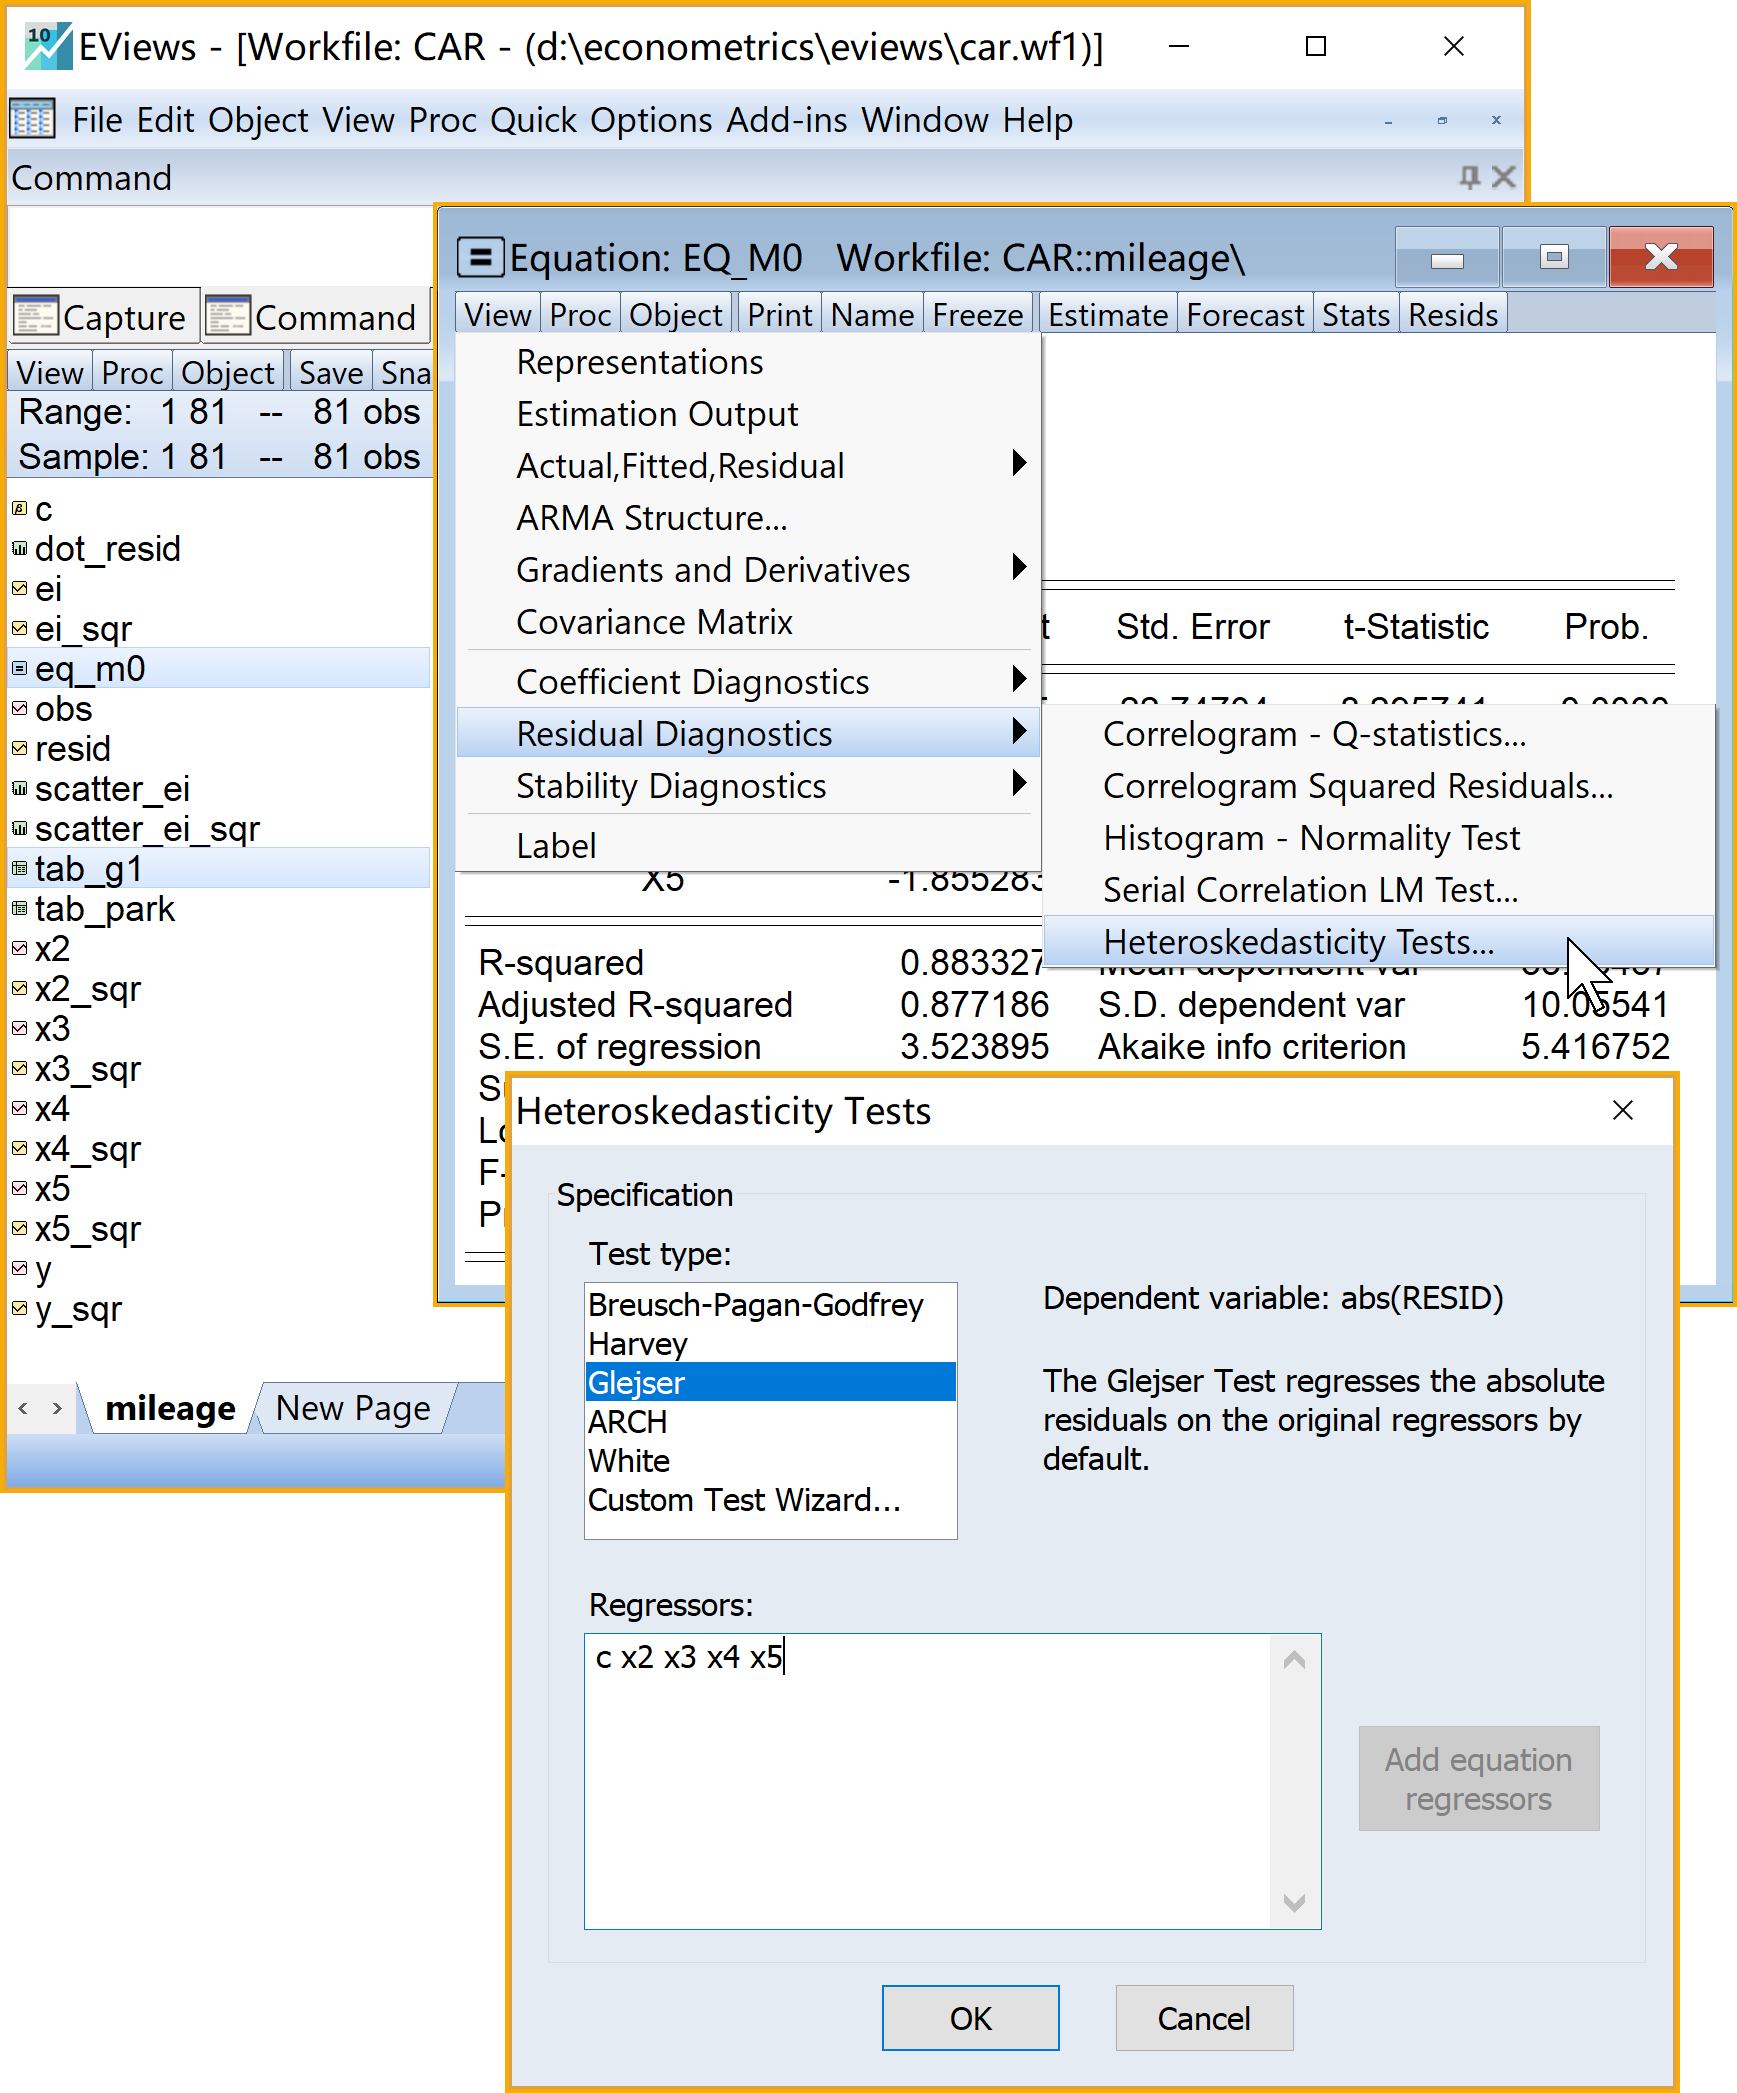
\includegraphics[width=24.12in]{picture/lab6-heteroskedasticity/4-test-G1-1} 

}

\caption{Glejser异方差检验操作1}\label{fig:fig-G1-test}
\end{figure}

\begin{figure}

{\centering 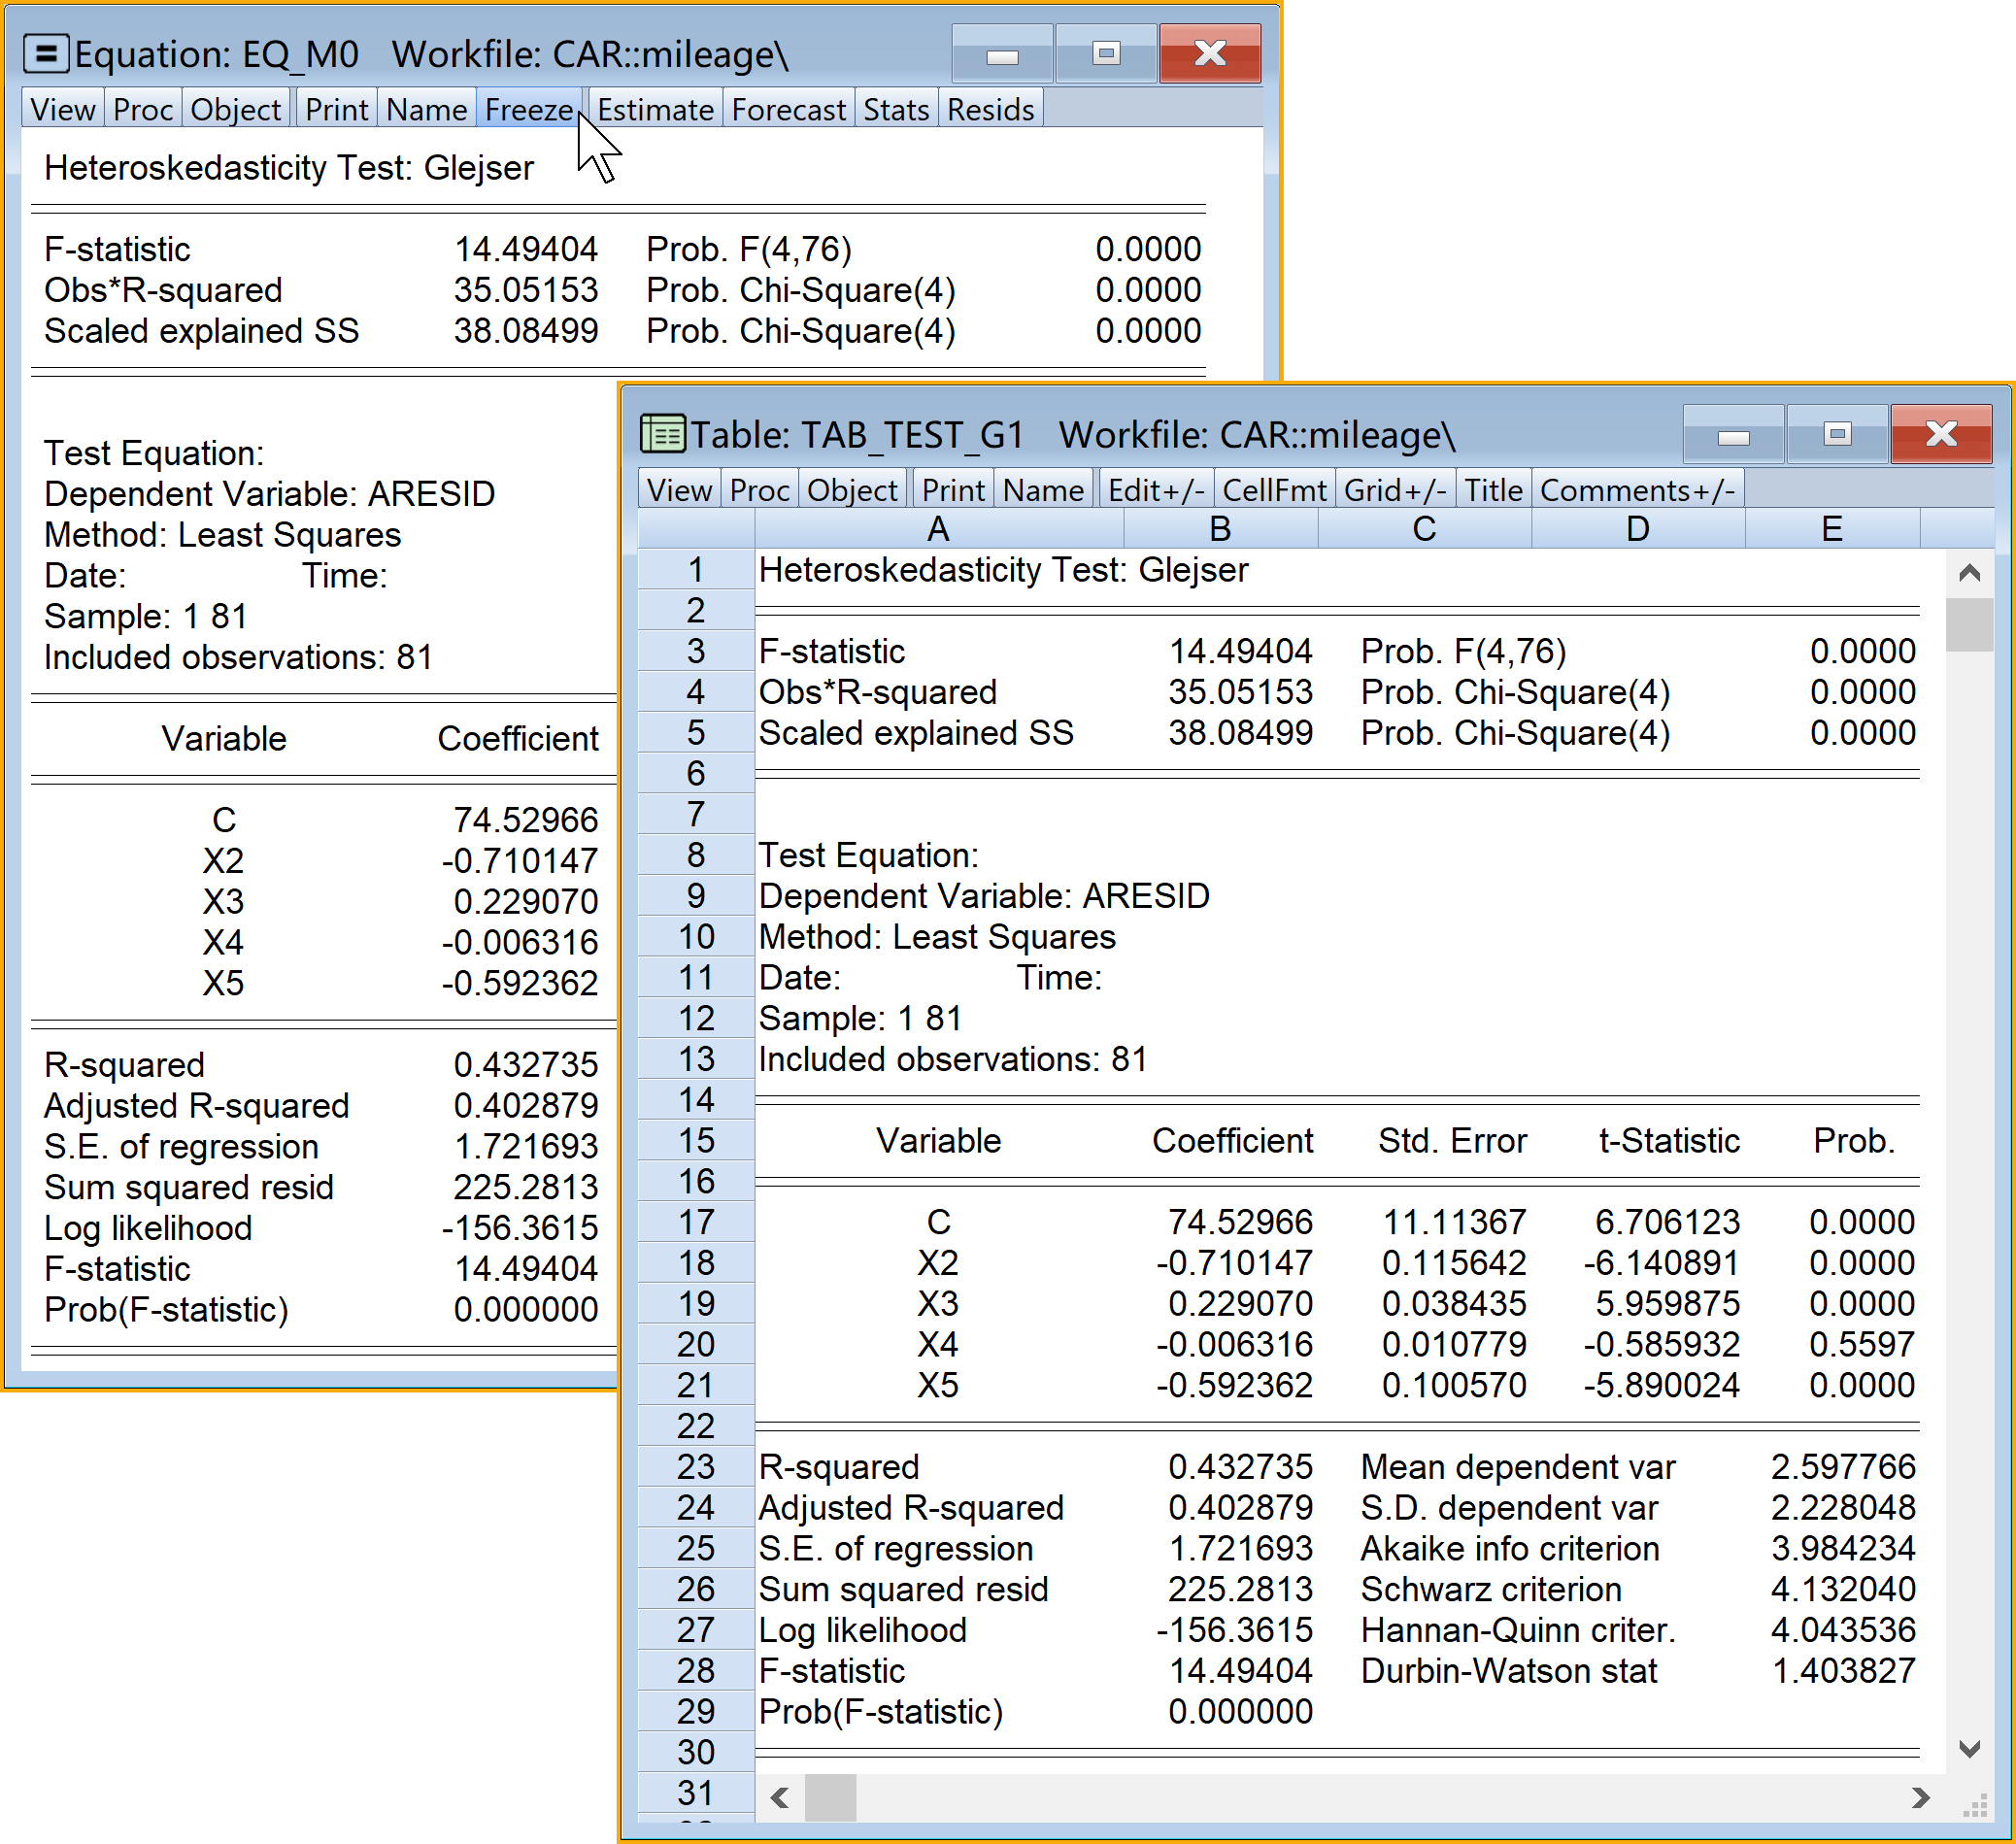
\includegraphics[width=28.83in]{picture/lab6-heteroskedasticity/4-test-G1-2} 

}

\caption{Glejser异方差检验报告1}\label{fig:fig-G1-report}
\end{figure}

\begin{itemize}
\tightlist
\item
  Eviews操作2(Glejser辅助方程\eqref{eq:G2},具体见图\ref{fig:fig-G2-test}):

  \begin{enumerate}
  \def\labelenumi{\arabic{enumi})}
  \tightlist
  \item
    打开主方程:双击方程(equation)对象
\includegraphics{picture/object/Equation.png}eq\_m0\\
  \item
    进入引导菜单:\(\Rightarrow\) View \(\Rightarrow\) Residual
    Diagnostics \(\Rightarrow\) Heteroskedasticity Test \(\Rightarrow\)
    Specification

    \begin{itemize}
    \tightlist
    \item
      设置诊断方法(Test type): 点击选择Glejser
    \item
      设置诊断方程(Regressors):输入c X2\^{}0.5 X3\^{}0.5 X4\^{}0.5
      X5\^{}0.5\\
    \end{itemize}
  \item
    完成设置:点击Ok\\
  \item
    命名并保存表格(table)对象
\includegraphics{picture/object/Table.png}

    \begin{itemize}
    \tightlist
    \item
      另存为表格(table)对象:点击Freeze
    \item
      命名并保存表格(table)对象:点击name(建议为tab\_G2)
    \item
      查看结果:双击
\includegraphics{picture/object/Table.png}tab\_G2
    \end{itemize}
  \end{enumerate}
\end{itemize}

具体Eviews报告见\ref{fig:fig-G2-report}:

\begin{figure}

{\centering 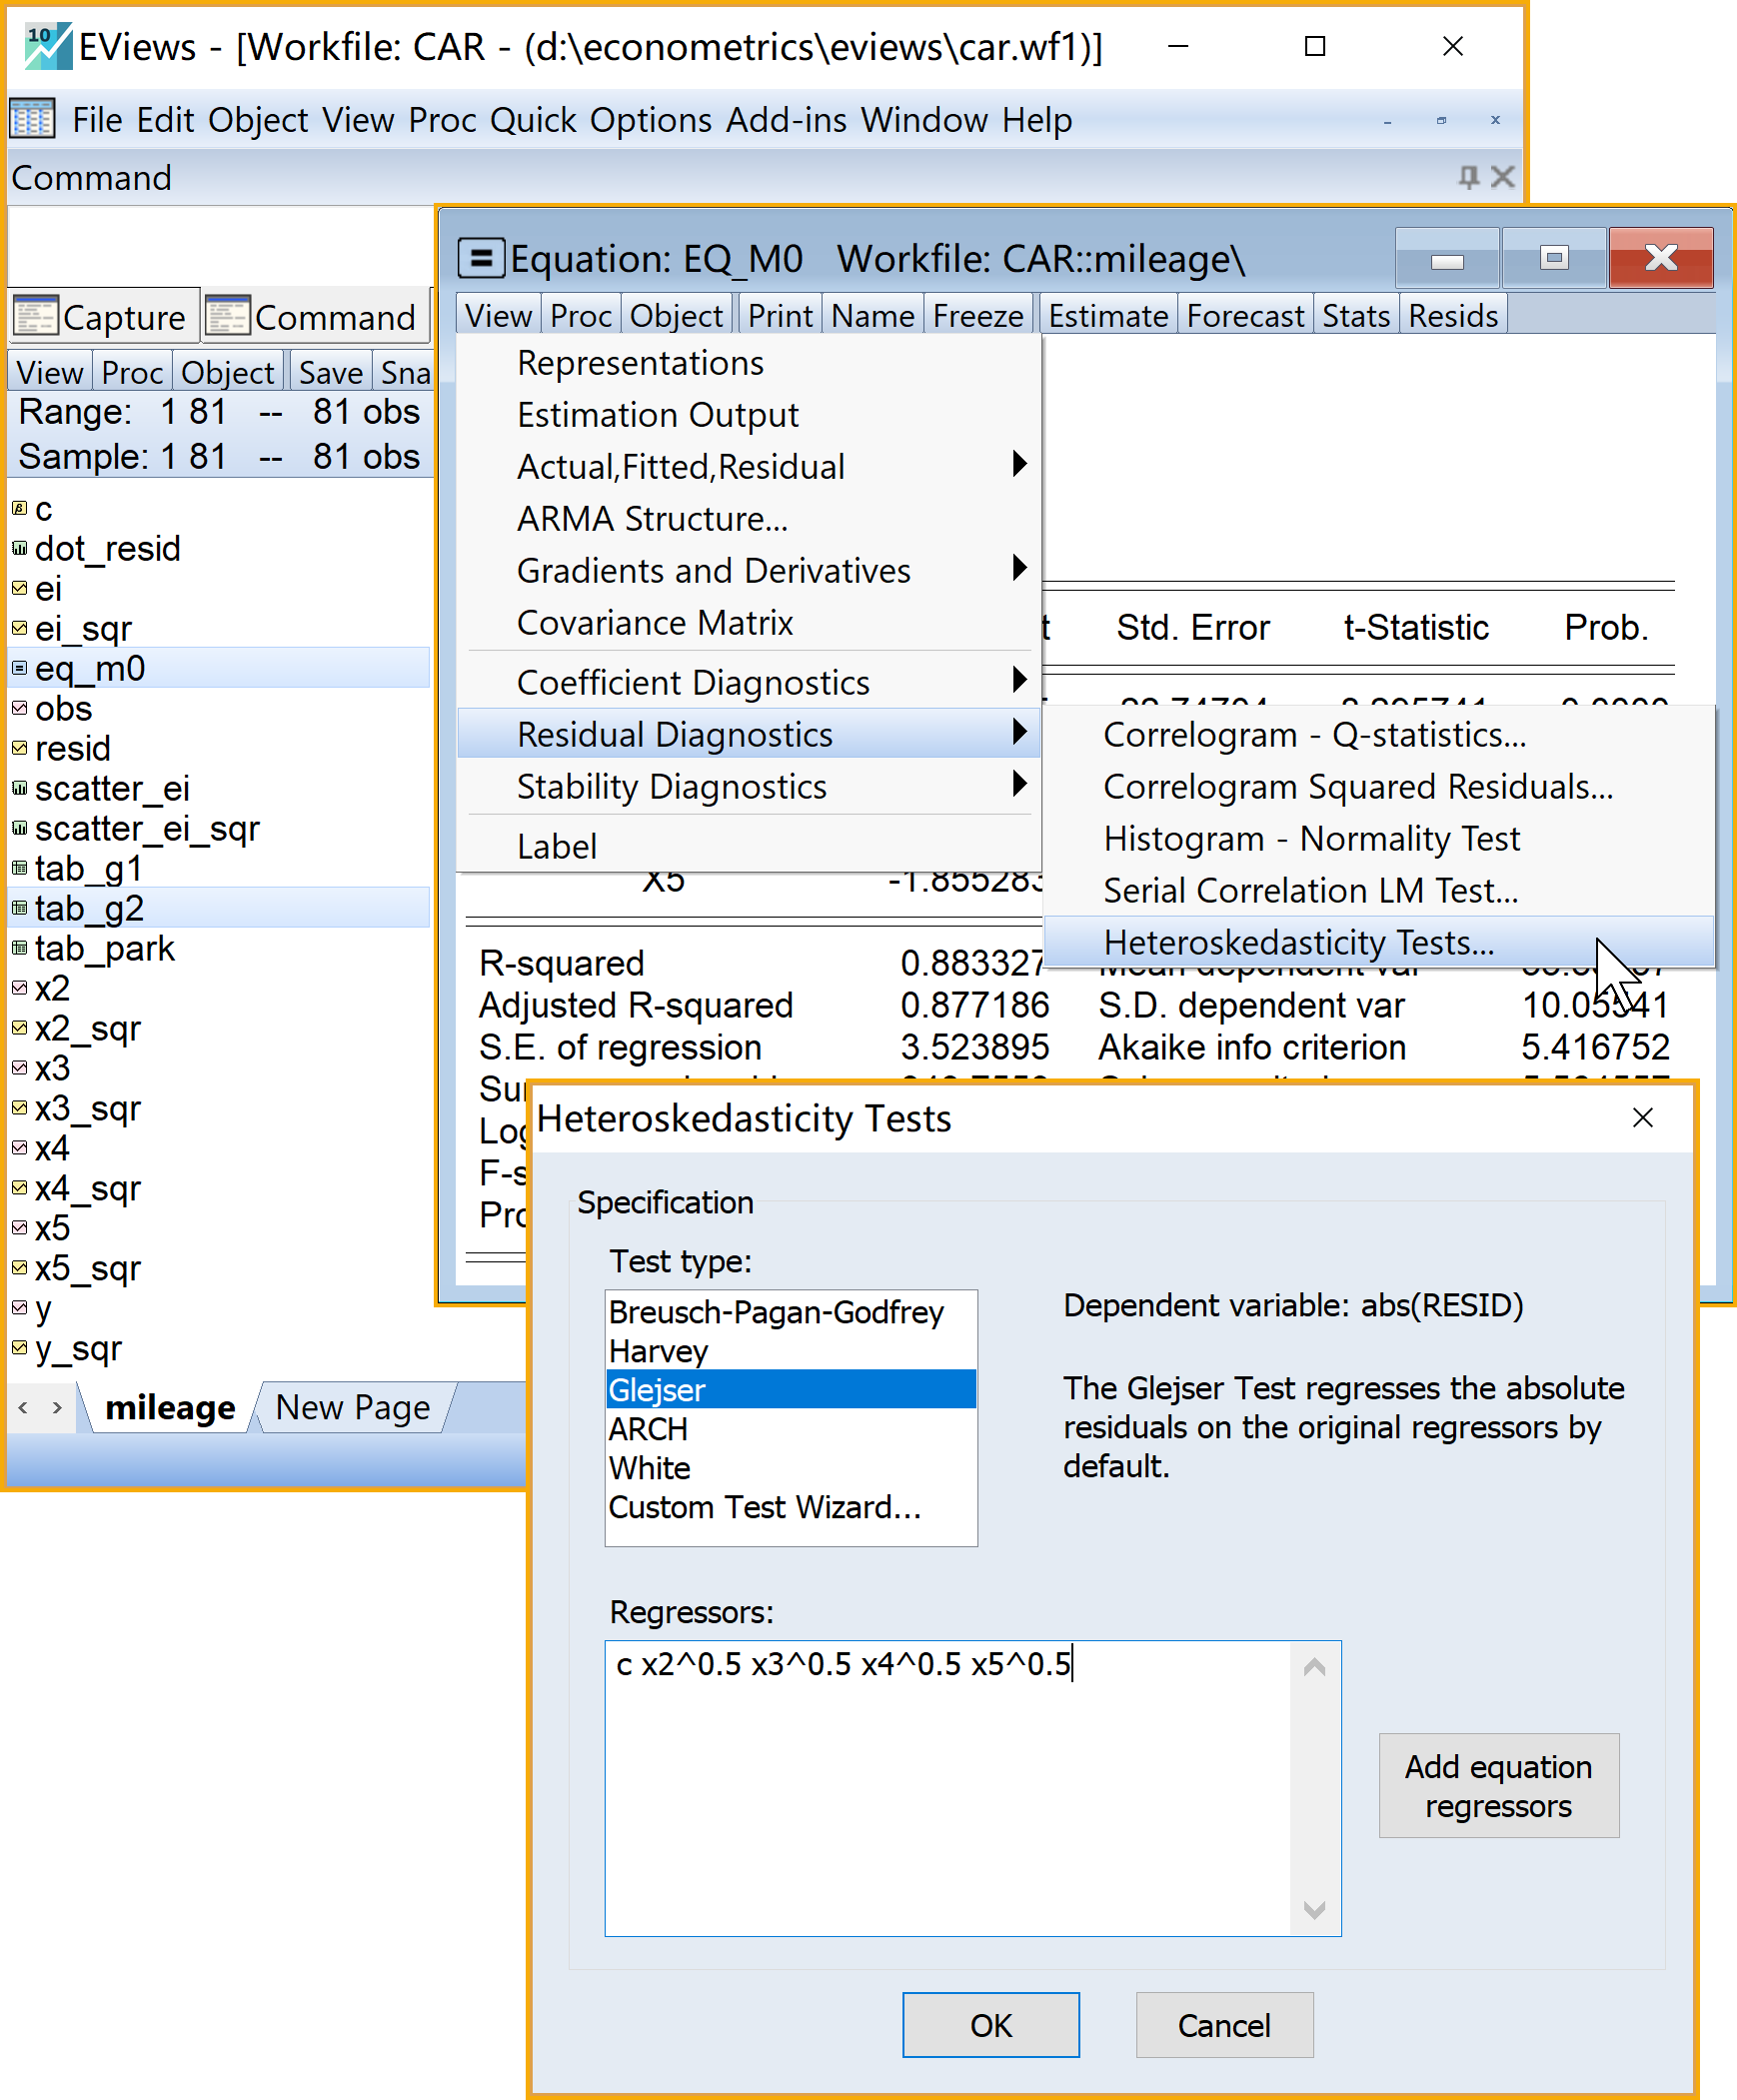
\includegraphics[width=24.14in]{picture/lab6-heteroskedasticity/4-test-G2-1} 

}

\caption{Glejser异方差检验操作2}\label{fig:fig-G2-test}
\end{figure}

\begin{figure}

{\centering 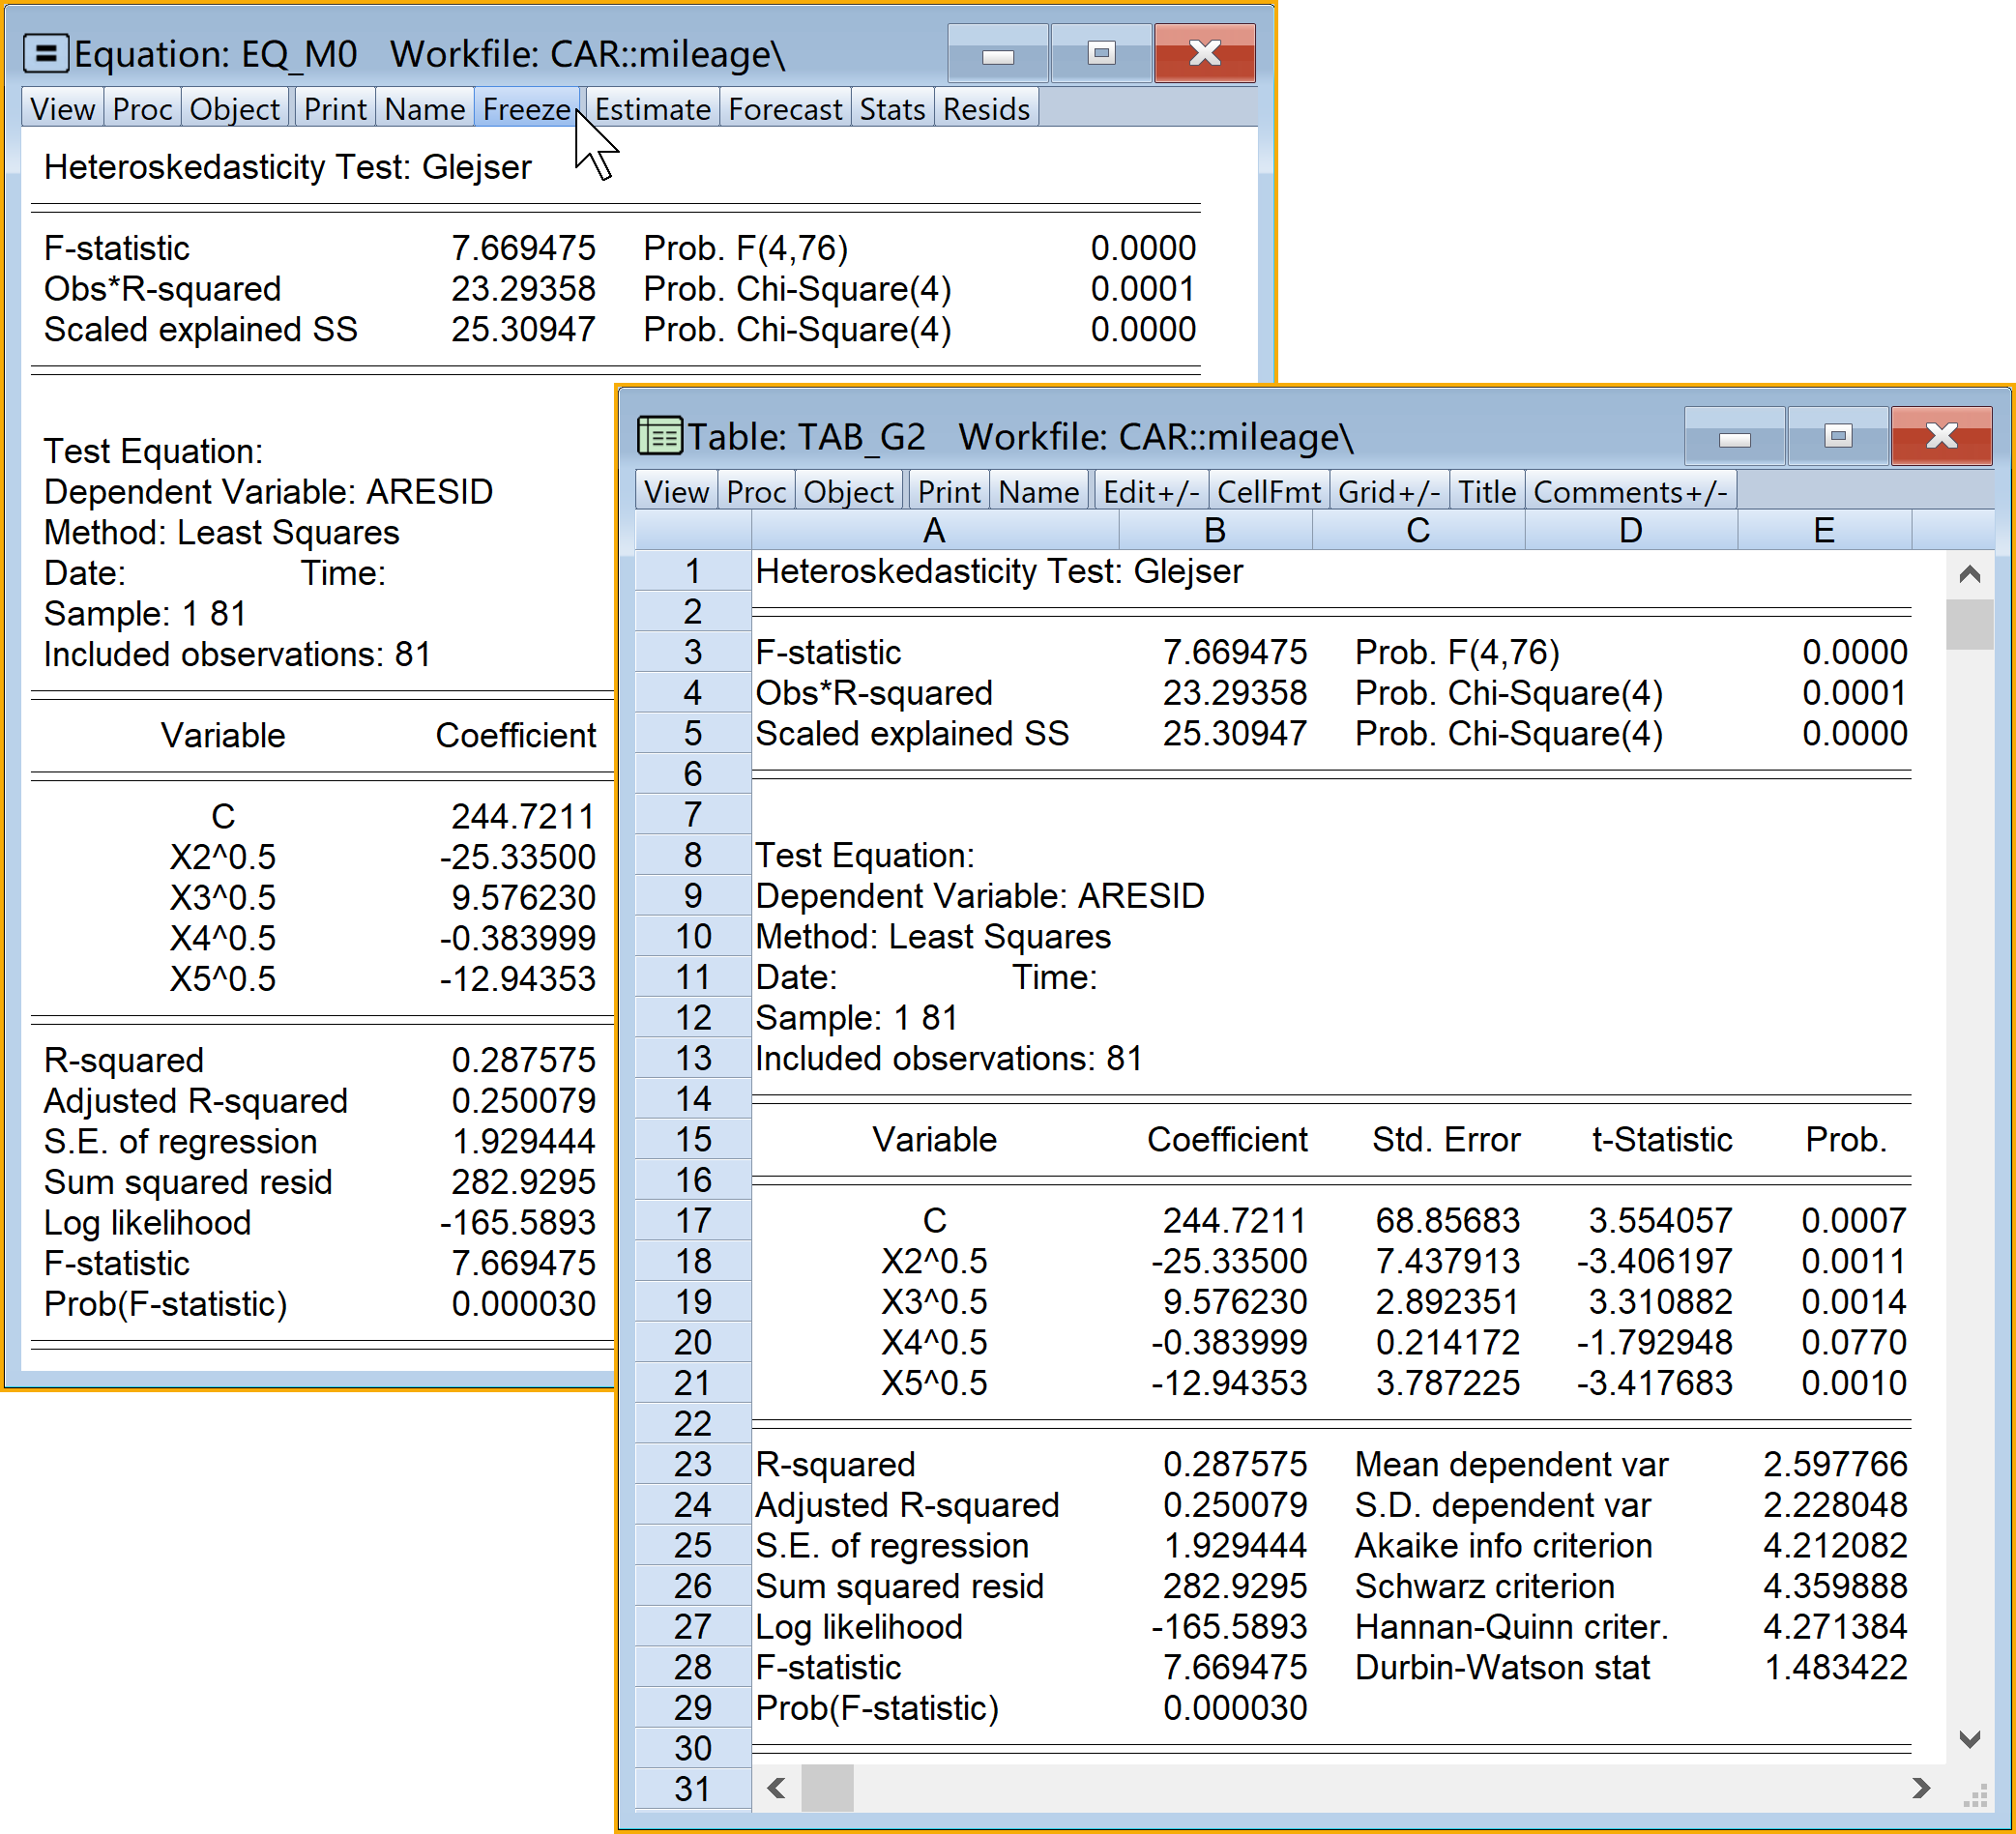
\includegraphics[width=28.96in]{picture/lab6-heteroskedasticity/4-test-G2-2} 

}

\caption{Glejser异方差检验报告2}\label{fig:fig-G2-report}
\end{figure}

\begin{itemize}
\tightlist
\item
  Eviews操作3(Glejser辅助方程\eqref{eq:G3},具体见图\ref{fig:fig-G3-test}):

  \begin{enumerate}
  \def\labelenumi{\arabic{enumi})}
  \tightlist
  \item
    打开主方程:双击方程(equation)对象\includegraphics{picture/object/Equation.png}eq\_m0\\
  \item
    进入引导菜单:\(\Rightarrow\) View \(\Rightarrow\) Residual
    Diagnostics \(\Rightarrow\) Heteroskedasticity Test \(\Rightarrow\)
    Specification

    \begin{itemize}
    \tightlist
    \item
      设置诊断方法(Test type): 点击选择Glejser
    \item
      设置诊断方程(Regressors):输入c 1/ X2 1/ X3 1/ X4 1/ X5\\
    \end{itemize}
  \item
    完成设置:点击Ok\\
  \item
    命名并保存表格(table)对象\includegraphics{picture/object/Table.png}

    \begin{itemize}
    \tightlist
    \item
      另存为表格(table)对象:点击Freeze
    \item
      命名并保存表格(table)对象:点击name(建议为tab\_G3)
    \item
      查看结果:双击\includegraphics{picture/object/Table.png}tab\_G3
    \end{itemize}
  \end{enumerate}
\end{itemize}

具体Eviews报告见\ref{fig:fig-G3-report}:

\begin{figure}

{\centering \includegraphics[width=24.11in]{picture/lab6-heteroskedasticity/4-test-G3-1} 

}

\caption{Glejser异方差检验操作3}\label{fig:fig-G3-test}
\end{figure}

\begin{figure}

{\centering \includegraphics[width=28.76in]{picture/lab6-heteroskedasticity/4-test-G3-2} 

}

\caption{Glejser异方差检验报告3}\label{fig:fig-G3-report}
\end{figure}

\hypertarget{bpg}{%
\subparagraph{BPG检验法}\label{bpg}}

\begin{itemize}
\tightlist
\item
  诊断辅助方程:
\end{itemize}

\begin{equation}
e^2_i=\hat{\alpha}_1+\hat{\alpha}_2X_{2i}+\cdots+\hat{\alpha}_kX_{ki}+v_i \label{eq:A-BPG} 
\end{equation}

\begin{itemize}
\tightlist
\item
  诊断标准:

  \begin{itemize}
  \tightlist
  \item
    如果诊断辅助方程\eqref{eq:A-BPG}的\(\chi^2\)检验(\texttt{scaled\ explained\ SS})\textbf{不显著}(对应的概率值P\textgreater{}0.1),则表明主模型\eqref{eq:M0-car}是同方差
  \item
    如果诊断辅助方程\eqref{eq:A-BPG}的\(\chi^2\)检验(\texttt{scaled\ explained\ SS})\textbf{显著}(对应的概率值P\textless{}0.1),则表明主模型\eqref{eq:M0-car}是异方差。
  \end{itemize}
\item
  Eviews操作(菜单操作实现,具体见图\ref{fig:fig-BPG-test}):

  \begin{enumerate}
  \def\labelenumi{\arabic{enumi})}
  \tightlist
  \item
    打开主方程:双击方程(equation)对象\includegraphics{picture/object/Equation.png}eq\_m0\\
  \item
    进入引导菜单:\(\Rightarrow\) View \(\Rightarrow\) Residual
    Diagnostics \(\Rightarrow\) Heteroskedasticity Test \(\Rightarrow\)
    Specification

    \begin{itemize}
    \tightlist
    \item
      设置诊断方法(Test type): 点击选择Breusch-Pagan-Godfrey
    \item
      设置诊断方程(Regressors):输入c X2 X3 X4 X5\\
    \end{itemize}
  \item
    完成设置:点击Ok\\
  \item
    命名并保存表格(table)对象\includegraphics{picture/object/Table.png}

    \begin{itemize}
    \tightlist
    \item
      另存为表格(table)对象:点击Freeze
    \item
      命名并保存表格(table)对象:点击name(建议为tab\_bpg)
    \item
      查看结果:双击\includegraphics{picture/object/Table.png}tab\_bpg
    \end{itemize}
  \end{enumerate}
\end{itemize}

具体Eviews报告见\ref{fig:fig-BPG-report}:

\begin{figure}

{\centering \includegraphics[width=24.11in]{picture/lab6-heteroskedasticity/4-test-BPG1} 

}

\caption{BPG异方差检验操作}\label{fig:fig-BPG-test}
\end{figure}

\begin{figure}

{\centering \includegraphics[width=29.25in]{picture/lab6-heteroskedasticity/4-test-BPG2} 

}

\caption{BPG异方差检验报告}\label{fig:fig-BPG-report}
\end{figure}

\hypertarget{white}{%
\subparagraph{White检验法}\label{white}}

\begin{itemize}
\tightlist
\item
  诊断辅助方程:
\end{itemize}

\begin{align}
Y_t & =\hat{\beta}_1+\hat{\beta}_2X_{2i}+\hat{\beta}_3X_{3i}+e_{i} \label{eq:M0-white} \\
e^2_i & =\hat{\alpha}_1+\hat{\alpha}_2X_{2i}+\hat{\alpha}_3X_{3i}+\hat{\alpha}_4X^2_{2i}+\hat{\alpha}_5X^2_{3i}+\hat{\alpha}_6X_{2i}X_{3i}+v_i \label{eq:A-white}
\end{align}

\begin{itemize}
\tightlist
\item
  诊断标准:

  \begin{itemize}
  \tightlist
  \item
    如果诊断辅助方程\eqref{eq:A-white}的\(\chi^2\)检验(\texttt{scaled\ explained\ SS})\textbf{不显著}(对应的概率值P\textgreater{}0.1),则表明主模型\eqref{eq:M0-white}是同方差
  \item
    如果诊断辅助方程\eqref{eq:A-white}的\(\chi^2\)检验(\texttt{scaled\ explained\ SS})\textbf{显著}(对应的概率值P\textless{}0.1),则表明主模型\eqref{eq:M0-white}是异方差。
  \end{itemize}
\item
  Eviews操作(菜单操作实现,具体见图\ref{fig:fig-white-test}):

  \begin{enumerate}
  \def\labelenumi{\arabic{enumi})}
  \tightlist
  \item
    打开主方程:双击方程(equation)对象\includegraphics{picture/object/Equation.png}eq\_m0\\
  \item
    进入引导菜单:\(\Rightarrow\) View \(\Rightarrow\) Residual
    Diagnostics \(\Rightarrow\) Heteroskedasticity Test \(\Rightarrow\)
    Specification

    \begin{itemize}
    \tightlist
    \item
      设置诊断方法(Test type): 点击选择White
    \item
      设置诊断方程(下面两类方程自行选择其一):

      \begin{itemize}
      \tightlist
      \item
        交叉项方程:\textbf{勾选} Include White cross term
      \item
        非交叉项方程:\textbf{不勾选} Include White cross term
      \end{itemize}
    \end{itemize}
  \item
    完成设置:点击Ok\\
  \item
    命名并保存表格(table)对象\includegraphics{picture/object/Table.png}

    \begin{itemize}
    \tightlist
    \item
      另存为表格(table)对象:点击Freeze
    \item
      命名并保存表格(table)对象:点击name(建议为tab\_white)
    \item
      查看结果:双击\includegraphics{picture/object/Table.png}tab\_white
    \end{itemize}
  \end{enumerate}
\end{itemize}

具体Eviews报告见\ref{fig:fig-white-report}:

\begin{figure}

{\centering \includegraphics[width=24.1in]{picture/lab6-heteroskedasticity/4-test-white1} 

}

\caption{White异方差检验报告操作}\label{fig:fig-white-test}
\end{figure}

\begin{figure}

{\centering \includegraphics[width=28.94in]{picture/lab6-heteroskedasticity/4-test-white2} 

}

\caption{White异方差检验报告}\label{fig:fig-white-report}
\end{figure}

\subsubsection{存在异方差问题的模型矫正}

\hypertarget{wls}{%
\paragraph{使用加权最小二乘法(WLS)矫正异方差问题}\label{wls}}

\hypertarget{wls1-sigma2_is2}{%
\subparagraph{\texorpdfstring{WLS矫正情形1:
方差\(\sigma^2_i\)已知且等于样本方差\(S^2\)}{WLS矫正情形1: 方差\textbackslash{}sigma\^{}2\_i已知且等于样本方差S\^{}2}}\label{wls1-sigma2_is2}}

\begin{itemize}
\tightlist
\item
  理论提示:
\end{itemize}

如果主模型\eqref{eq:M0-car}存在异方差问题,且假设方差正比于样本方差\(S^2_i\),则有:

\begin{equation}
var(u_i)=E(u^2_i)=\sigma^2_i=\sigma^2S^2_i \label{eq:WLS-S2}
\end{equation}

对主模型\eqref{eq:M0-car}两边同时除以\(S_i\),得到:

\begin{align}
\frac{Y_i}{S_i} &=\frac{\hat{\beta}_1}{S_i}+\hat{\beta}_2\frac{X_{2i}}{S_i}+\hat{\beta}_3\frac{X_{3i}}{S_i}+\hat{\beta}_4\frac{X_{4i}}{S_i}+\hat{\beta}_5\frac{X_{5i}}{S_i}+\frac{e_{i}}{S_i}\label{eq:WLS-S2-adj}\\
Y^{\ast}_i &=\beta^{\ast}_1+\beta^{\ast}_2X^{\ast}_{2i}+\beta^{\ast}_3X^{\ast}_{3i}+\beta^{\ast}_4X^{\ast}_{4i}+\beta^{\ast}_5X^{\ast}_{5i}+v_{i} \label{eq:WLS1-S2-red} 
\end{align}

\hypertarget{wls2-sigma2_ix2_i}{%
\subparagraph{\texorpdfstring{WLS矫正情形2:
方差\(\sigma^2_i\)正比于\(X^2_i\)}{WLS矫正情形2: 方差\textbackslash{}sigma\^{}2\_i正比于X\^{}2\_i}}\label{wls2-sigma2_ix2_i}}

\begin{itemize}
\tightlist
\item
  理论提示:
\end{itemize}

如果主模型\eqref{eq:M0-car}存在异方差问题,且假设方差正比于\(X^2_i\),则有:

\begin{equation}
var(u_i)=E(u^2_i)=\sigma^2_i=\sigma^2X^2_i \label{eq:WLS-X2}
\end{equation}

对主模型\eqref{eq:M0-car}两边同时除以\(X_i\),得到:

\begin{align}
\frac{Y_i}{X_{2i}} &=\frac{\hat{\beta}_1}{X_{2i}}+\hat{\beta}_2+\hat{\beta}_3\frac{X_{3i}}{X_{2i}}+\hat{\beta}_4\frac{X_{4i}}{X_{2i}}+\hat{\beta}_5\frac{X_{5i}}{X_{2i}}+\frac{e_{i}}{X_{2i}}\label{eq:WLS-X2-adj}\\
Y^{\ast}_i &=\beta^{\ast}_1+\beta^{\ast}_2X^{\ast}_{2i}+\beta^{\ast}_3X^{\ast}_{3i}+\beta^{\ast}_4X^{\ast}_{4i}+\beta^{\ast}_5X^{\ast}_{5i}+v_{i} \label{eq:WLS1-X2-red}
\end{align}

\begin{itemize}
\tightlist
\item
  Eviews操作:
\end{itemize}

\hypertarget{wls3-sigma2_ix_i}{%
\subparagraph{\texorpdfstring{WLS矫正情形3:
方差\(\sigma^2_i\)正比于\(X_i\)}{WLS矫正情形3: 方差\textbackslash{}sigma\^{}2\_i正比于X\_i}}\label{wls3-sigma2_ix_i}}

\begin{itemize}
\tightlist
\item
  理论提示:
\end{itemize}

如果主模型\eqref{eq:M0-car}存在异方差问题,且假设方差正比于\(X_i\),则有:

\begin{equation}
var(u_i)=E(u^2_i)=\sigma^2_i=\sigma^2X_i \label{eq:WLS-X}
\end{equation}

对主模型\eqref{eq:M0-car}两边同时除以\(\sqrt{X_i}\),得到:

\begin{align}
\frac{Y_i}{\sqrt{X_i}} &=\frac{\hat{\beta}_1}{\sqrt{X_i}}+\hat{\beta}_2\sqrt{X_i}+\hat{\beta}_3\frac{X_{3i}}{\sqrt{X_i}}+\hat{\beta}_4\frac{X_{4i}}{\sqrt{X_i}}+\hat{\beta}_5\frac{X_{5i}}{\sqrt{X_i}}+\frac{e_{i}}{\sqrt{X_i}}\label{eq:WLS1-adj}\\
Y^{\ast}_i &=\beta^{\ast}_1+\beta^{\ast}_2X^{\ast}_{2i}+\beta^{\ast}_3X^{\ast}_{3i}+\beta^{\ast}_4X^{\ast}_{4i}+\beta^{\ast}_5X^{\ast}_{5i}+v_{i} \label{eq:WLS1-red}
\end{align}

\hypertarget{wls4-sigma2_ihaty_i2}{%
\subparagraph{\texorpdfstring{WLS矫正情形4:
方差\(\sigma^2_i\)正比于\(\hat{Y_i}^2\)}{WLS矫正情形4: 方差\textbackslash{}sigma\^{}2\_i正比于\textbackslash{}hat\{Y\_i\}\^{}2}}\label{wls4-sigma2_ihaty_i2}}

\begin{itemize}
\tightlist
\item
  理论提示:
  如果主模型\eqref{eq:M0-car}存在异方差问题,且假设方差正比于\(\hat{Y_i}^2\),则有:
\end{itemize}

\begin{equation}
var(u_i)=E(u^2_i)=\sigma^2_i=\sigma^2\hat{Y_i}^2 \label{eq:WLS-Y2}
\end{equation}

对主模型\eqref{eq:M0-car}两边同时除以\(\hat{Y_i}\),得到:

\begin{align}
\frac{Y_i}{\hat{Y_i}} &=\frac{\hat{\beta}_1}{\hat{Y_i}}+\hat{\beta}_2\frac{X_{2i}}{\hat{Y_i}}+\hat{\beta}_3\frac{X_{3i}}{\hat{Y_i}}+\hat{\beta}_4\frac{X_{4i}}{\hat{Y_i}}+\hat{\beta}_5\frac{X_{5i}}{\hat{Y_i}}+\frac{e_{i}}{\hat{Y_i}}\label{eq:WLS-Y2-adj}\\
Y^{\ast}_i &=\beta^{\ast}_1+\beta^{\ast}_2X^{\ast}_{2i}+\beta^{\ast}_3X^{\ast}_{3i}+\beta^{\ast}_4X^{\ast}_{4i}+\beta^{\ast}_5X^{\ast}_{5i}+v_{i} \label{eq:WLS1-Y2-red}
\end{align}

\begin{itemize}
\tightlist
\item
  Eviews操作:
\end{itemize}

\hypertarget{wls5-sigma2_i}{%
\subparagraph{\texorpdfstring{WLS矫正情形5:
方差\(\sigma^2_i\)未知}{WLS矫正情形5: 方差\textbackslash{}sigma\^{}2\_i未知}}\label{wls5-sigma2_i}}

\begin{itemize}
\tightlist
\item
  理论提示:
  如果主模型\eqref{eq:M0-car}存在异方差问题,且假设方差正比于\(\hat{Y_i}^2\),则有:
\end{itemize}

\begin{equation}
var(u_i)=E(u^2_i)=\sigma^2_i=\sigma^2\hat{Y_i}^2 \label{eq:WLS-Y2}
\end{equation}

对主模型\eqref{eq:M0-car}两边同时取对数\(ln()\),得到:

\begin{equation}
ln{Y_t} =\hat{\beta}_1+\hat{\beta}_2ln{X_{2i}}+\hat{\beta}_ln{3X_{3i}}+\hat{\beta}_4ln{X_{4i}}+\hat{\beta}_5ln{X_{5i}}+e_{i} \label{eq:WLS-ln}
\end{equation}

\hypertarget{white}{%
\paragraph{使用White校正法矫正异方差问题}\label{white}}

\begin{itemize}
\item
  理论提示
\item
  Eviews操作(见图\ref{fig:fig-adj-white})

  \begin{enumerate}
  \def\labelenumi{\arabic{enumi})}
  \tightlist
  \item
    依次选择\(\Rightarrow\) Quick \(\Rightarrow\) Estimation Equation\\
  \item
    引导设置Equation Estimation \(\Rightarrow\) Specification

    \begin{enumerate}
    \def\labelenumii{\alph{enumii}.}
    \tightlist
    \item
      方程设置(Equation Specification): Y
      (此处如果仅填Y变量,则任何X变量都没有强制一定要留在模型中)
    \item
      输入自变量(List of search regressors):Y c X2 X3 X4 X5
    \item
      估计方法(Estimation settings):

      \begin{itemize}
      \tightlist
      \item
        Method:选择\texttt{LS\ -\ Least\ Squares(NLS\ and\ ARMA)}
      \item
        Sample: \textbf{默认设置}
      \end{itemize}
    \end{enumerate}
  \item
    引导设置Equation Estimation \(\Rightarrow\) Options

    \begin{enumerate}
    \def\labelenumii{\alph{enumii}.}
    \tightlist
    \item
      系数协方差设置(Coefficient covariance)

      \begin{itemize}
      \tightlist
      \item
        协方差方法(Coefficient method):下拉选择Huber-White
      \end{itemize}
    \item
      权重设置(Weights):默认设置
    \item
      最优化设置(Optimization):默认设置
    \item
      完成设置:点击\texttt{OK}\\
    \end{enumerate}
  \item
    模型命名:建议为\texttt{eq\_adj\_white}\\
  \item
    查看分析报告(见图\ref{fig:fig-adj-white-report})
  \end{enumerate}
\end{itemize}

\begin{figure}

{\centering \includegraphics[width=24.92in]{picture/lab6-heteroskedasticity/5-adj-white1} 

}

\caption{White异方差矫正法的操作}\label{fig:fig-adj-white}
\end{figure}

\begin{figure}

{\centering \includegraphics[width=18.53in]{picture/lab6-heteroskedasticity/5-adj-white2} 

}

\caption{White异方差矫正法的Eviews报告}\label{fig:fig-adj-white-report}
\end{figure}

\subsection{作业题}

\textbf{财富500强企业高管薪水数据}:表\ref{tab:data-salary}给出给出了447辆汽车在Y高管薪水及分红,X2担任
CEO年数(不足6个月视为的0),X3总裁CEO的年龄,X4企业的总销售收入,X5企业的利润,X6企业的总资产等方面的数据。

\begin{table}

\caption{\label{tab:data-salary}财富500强企业高管薪水数据(n=447)}
\centering
\begin{tabular}[t]{rrrrrrr}
\toprule
obs & Y & X2 & X3 & X4 & X5 & X6\\
\midrule
1 & 3030 & 7 & 61 & 161315 & 2956.0 & 257389\\
2 & 6050 & 0 & 51 & 144416 & 22071.0 & 237545\\
3 & 3571 & 11 & 63 & 139208 & 4430.0 & 49271\\
4 & 3300 & 6 & 60 & 100697 & 6370.0 & 92630\\
5 & 10000 & 18 & 63 & 100469 & 9296.0 & 355935\\
\addlinespace
443 & 1866 & 10 & 59 & 2934 & 375.0 & 35800\\
444 & 906 & 6 & 59 & 2933 & 193.9 & 4986\\
445 & 2300 & 9 & 57 & 2910 & 182.9 & 2739\\
446 & 875 & 7 & 50 & 2905 & 132.0 & 5009\\
447 & 1758 & 5 & 62 & 2896 & 16.6 & 2855\\
\bottomrule
\end{tabular}
\end{table}

变量说明见表\ref{tab:label-salary}:

\begin{table}

\caption{\label{tab:label-salary}变量定义及说明}
\centering
\begin{tabular}[t]{l|l}
\hline
variable & label\\
\hline
obs & TOP500公司序号\\
\hline
Y & 高管薪水及分红\\
\hline
X2 & 担任 CEO年数(不足6个月视为的0)\\
\hline
X3 & 总裁CEO的年龄\\
\hline
X4 & 企业的总销售收入\\
\hline
X5 & 企业的利润\\
\hline
X6 & 企业的总资产\\
\hline
\end{tabular}
\end{table}

请考虑如下样本回归模型:

\begin{equation}
Y_i=\beta_1+\beta_2X_{2i}+\beta_3X_{3i}+\beta_4X_{4i}+\beta_5X_{5i}+\beta_6X_{6i}+e_{i} \label{eq:M0-salary}
\end{equation}

请回答如下问题:

\begin{enumerate}
\def\labelenumi{\arabic{enumi}.}
\tightlist
\item
  根据回归模型\eqref{eq:M0-salary},写出总体回归模型(PRM),并对参数的理论预期(符号、大小、关系)进行说明。\\
\item
  利用Eviews对样本回归模型\eqref{eq:M0-salary}进行回归分析(将报告截图过来,并写出相应的简要报告形式------三行式或四行式)。参数估计结果符合你的理论预期么?\\
\item
  回归模型\eqref{eq:M0-salary}存在异方差问题的证据吗?请以此按照下列方法进行诊断,并分别得到分析结论(要求截图过来并进行简要说明):

  \begin{enumerate}
  \def\labelenumii{\alph{enumii}.}
  \tightlist
  \item
    非正式检验法(图解法):

    \begin{itemize}
    \tightlist
    \item
      绘制\(e_i\)序列和\(e^2_i\)序列的描点图(dot
      plot),得到你的初步结论。\\
    \item
      分别绘制\(e_i\)序列分别与\(Y_i\)、\(X_i(i=2,\cdots,6\)序列的散点图(scatter
      plot),得到你的初步结论\\
    \item
      分别绘制\(e^2_i\)与\(Y^2_i\)、\(X^2_i(i=2,\cdots,6\)序列的散点图(scatter
      plot),得到你的初步结论\\
    \end{itemize}
  \item
    正式检验法

    \begin{itemize}
    \tightlist
    \item
      利用Park检验法,并得出你的初步结论(要求写出park诊断方程,并将park检验结果截图过来)\\
    \item
      利用Glejser检验法,并得出你的初步结论(请确定X,并做三个类型的辅助回归。分别将Glejser检验结果截图过来)
    \end{itemize}
  \end{enumerate}
\end{enumerate}

\begin{align}
|e_i| & =\hat{\alpha}_1+\hat{\alpha}_2X_{2i}+\cdots+\hat{\alpha}_kX_{ki}+v_i &&\text{G1} \\
|e_i| & =\hat{\alpha}_1+\hat{\alpha}_2\sqrt{X_{2i}}+\cdots+\hat{\alpha}_k\sqrt{X_{ki}}+v_i &&\text{G2} \\
|e_i| & =\hat{\alpha}_1+\hat{\alpha}_2\frac{1}{X_{2i}}+\cdots+\hat{\alpha}_k\frac{1}{X_{ki}}+v_i &&\text{G3} 
\end{align}

\begin{enumerate}
\def\labelenumi{\arabic{enumi}.}
\setcounter{enumi}{2}
\item
  \begin{enumerate}
  \def\labelenumii{\alph{enumii}.}
  \setcounter{enumii}{1}
  \item
    \begin{itemize}
    \tightlist
    \item
      利用BPG检验法,并得出你的初步结论(要求写出BPG诊断方程,并将BPG检验结果截图过来)\\
    \item
      利用White检验法(注意交叉项的使用),并得出你的初步结论(要求写出White诊断方程,并将White检验结果截图过来)\\
    \end{itemize}
  \end{enumerate}
\item
  若发现存在异方差问题,你如何进行纠正主模型\eqref{eq:M0-salary}?

  \begin{enumerate}
  \def\labelenumii{\alph{enumii}.}
  \tightlist
  \item
    使用White校正法纠正异方差问题,并比较与主模型\eqref{eq:M0-salary}的差别。(要求分别截图两个回归方程的Eviews报告,进行对照分析并得到结论)\\
  \item
    使用加权最小二乘法纠正异方差问题(提醒:根据前述分析,几种处理方法选择一种合适的处理方法,进行模型矫正分析。请说明你选择这种处理办法的理由,并得到分析结论!)\\
  \end{enumerate}
\item
  现在做以
  \(ln(Y_i)\)为因变量的第二个模型。异方差性有所改善吗?(要求截图相关Eviews报告,并简要陈述理由)。
\end{enumerate}


\end{document}
